\documentclass{mimosis}
\graphicspath{ {./Figures/} }
\usepackage{float}
\usepackage{setspace}
%\usepackage{cite}


% letter size
\KOMAoptions{paper=letter}

\newglossaryentry{LaTeX}{%
  name        = {\LaTeX},
  description = {A document preparation system},
  sort        = {LaTeX},
}

\newglossaryentry{Real numbers}{%
  name        = {$\real$},
  description = {The set of real numbers},
  sort        = {Real numbers},
}
\newacronym[description={Principal component analysis}]{PCA}{PCA}{principal component analysis}
\newacronym[description={Topological data analysis}]   {TDA}{TDA}{topological data analysis}
\newacronym[description={Canada Basin Acoustic Propagation Experiment}]   {CANAPE}{CANAPE}{Canada Basin Acoustic Propagation Experiment}
\newacronym[description={Ambient Noise Level}]   {ANL}{ANL}{Ambient Noise Level}
\newacronym[description={European Organisation for the Exploitation of Meteorological Satellites}]   {EUMETSAT}{EUMETSAT}{European Organisation for the Exploitation of Meteorological Satellites}
\newacronym[description={Ocean and Sea Ice Satellite Application Facility}]   {OSI SAF}{OSI SAF}{Ocean and Sea Ice Satellite Application Facility}
\newacronym[description={Danes}]   {DMI}{DMI}{Danish Meteorological Institute}
\newacronym[description={dB}]   {dB}{dB}{decibel}
\newacronym[description={pdf}]   {PDF}{PDF}{Probability Density Function}



\makeindex
\makeglossaries
	\doublespacing
	
%%%%%%%%%%%%%%%%%%%%%%%%%%%%%%%%%%%%%%%%%%%%%%%%%%%%%%%%%%%%%%%%%%%%%%%%
% Title Page Information
%%%%%%%%%%%%%%%%%%%%%%%%%%%%%%%%%%%%%%%%%%%%%%%%%%%%%%%%%%%%%%%%%%%%%%%%

\title{\textbf{Oceanic ambient noise in the Arctic on the Chukchi Shelf}} % due by jul 15
\author{LTJG Kathryn Fung}
\date{August 6, 2022}

\begin{document}

% no frontmatter b/c MIT wants consecutively Arabic numbered pages
\mainmatter
  \def\signature#1#2{\par\noindent#1\dotfill\null\\*
  {\raggedleft #2\par}}

%% --- TITLEPAGE --- %%

% keep this to protect internal macros + use @ as a normal character
\makeatletter

\begin{titlepage}
  \begin{center}
    \begin{Large}
      \@title
    \end{Large}\\[0.1em]
    %
    \emph{\footnotesize by}\\
    {\large \@author} \\[-0.25em]
    B.S.E. 2020, Ocean Engineering, \textsc{United States Naval Academy} \\ [2em]
    %
    \begin{singlespace}
    {Submitted to the Joint Program in Oceanography and Applied Ocean Science \& Engineering in partial fulfillment of the requirements for the degree of Doctor of Philosophy in Mechanical \& Oceanographic Engineering} \\
    \end{singlespace}
    %
    \emph{\footnotesize at the}\\
    {\large \textsc{Massachusetts Institute of Technology}} \\
    \emph{\footnotesize and the}\\
    {\large \textsc{Woods Hole Oceanographic Institution}} \\ [2em]
    %
    \begin{singlespace}
    {\copyright2022 K. Fung. All rights reserved. \\ The author hereby grants to MIT and WHOI permission to reproduce and to distribute publicly copies of this thesis document in whole or in part in any medium now known or hereafter created.} \\ [2em]

    \signature{Author}{\small Department of Mechanical Engineering, MIT \\ Applied Ocean Science \& Engineering, WHOI \\ \@date}
    \vspace{1em}
    \signature{Certified by}{Julien Bonnel \\ \small Professor of Mechanical and Ocean Engineering, MIT \\ Thesis Supervisor}
    \vspace{1em}
    \signature{Accepted by}{Evelyn Wang \\ \small Professor of Mechanical Engineering, MIT \\ Chair, Department Committee on Graduate Students}
    \vspace{1em}
    \signature{Accepted by}{Weifang Gordon Zhang \\ \small Associate Scientist with Tenure, Applied Ocean Physics \& Engineering, WHOI \\ Chair, Joint Committee for Applied Ocean Science \& Engineering}
    \end{singlespace}
  \end{center}
  \makeatother
\end{titlepage}

\newpage
\null
\thispagestyle{empty}
\newpage
  %% ABSTRACT %%
\begin{center}
{\large \@title} \\
\emph{\footnotesize by} \\
\@author \\
\end{center}

\vspace{-1em}

\begin{center}
\begin{singlespace}
{\parindent0pt
\small
Submitted to the Department of Mechanical Engineering and the Joint Program in Applied Ocean Science and Engineering on \@date ~in partial fulfillment of the requirements for the degree of Master of Science in Mechanical Engineering}
\end{singlespace}
\end{center}

\begin{singlespace}
{\parindent0pt 
	{\large \textsc{Abstract}} \\ %less than 200 words for WHOI (350 for MIT) 
	% 154 words
This thesis encompasses an analysis of underwater ambient noise collected by the yearlong Canada Basin Acoustic Propagation Experiment (CANAPE) on the Chukchi Shelf of the Arctic. This location contained the Beaufort Duct, a significant effect of climate change on the Arctic's underwater soundscape. A study of the statistical and probability metrics was conducted on a frequency band of 50-1900 Hz to examine the relation between environmental drivers and noise patterns. The presence of ice typically decreases broadband ambient noise, when compared to ice-free seas. However, the Beaufort Duct under ice increases the ambient noise levels below 1 kHz. The relationship between ambient noise and the environment is further explored by studying the link between distant ice movements and ambient levels Correlation between the two is found to exist from 300-1500 Hz, as distant (1200 km) ice drift motion appears to drive noise levels at the receiver. [Work supported by the Office of Naval Research]

	\noindent Thesis Supervisor: Dr. Julien Bonnel \\
	\noindent Title: Associate Scientist, WHOI \\
}
\end{singlespace}

\newpage
\null
\thispagestyle{empty}
\newpage
  
\noindent
\begin{singlespace}
{\parindent0pt
	{\large \textsc{Acknowledgments}} \\

	Acknowledgments here.

	This thesis was produced thanks to generous help and support from an abundance of sources, from MIT, WHOI, and outside the institutions. A special thanks to my advisor, Dr. Julien Bonnel for unexpectedly taking me on as his first Navy student when circumstances arose, giving me an interesting project, and reading all of my confusing words. For all those who made CANAPE possible, I hope that my work helps to further the purposes of the project. I also appreciate the support of so many fellow students and family members who helped me get through the difficult first years of MIT-online due to COVID-19. A shout out to Dr. Mike Benjamin for making the most interesting and entertaining class I've ever taken through a laptop, and for approving all my courses. And thank you to Dr. Erin Fischell for welcoming me into the Joint Program in such un-normal times. Funding sources include the Navy and Office of Naval Research. The funding for the collection of the acoustic data came from ONR under grant number N00014-15-1-2196 (Principal Investigator: Y.-T. Lin, WHOI).
}

\end{singlespace}

\newpage
\null
\thispagestyle{empty}
\newpage

  \tableofcontents
  \listoffigures
  \listoftables
  
  % table of contents
  
%%%%%%%%%%%%%%%%%%%%%%%%%%%%%%%%%%%%%%%%%%%%%%%%%%%%%%%%%%%%%%%%%%%%%%%%
\chapter{Introduction}  \label{introduction}
%%%%%%%%%%%%%%%%%%%%%%%%%%%%%%%%%%%%%%%%%%%%%%%%%%%%%%%%%%%%%%%%%%%%%%%%

\begin{center}
  \begin{minipage}{0.5\textwidth}
    \begin{small}
      "Some say the world will end in fire, some say in ice." 
      
      ― Robert Frost
    \end{small}
  \end{minipage}
  \vspace{0.5cm}
\end{center}

\noindent Though the world knows by now that global climate change is a practically unstoppable force that will eventually dramatically affect humanity and our world, exactly how it affects this future is not known yet. Is a widely documented and proven phenomena, the resultant effects of it on the natural world that we inhabit is still an ongoing mystery, but one that can be investigated in the present. 

%%%%%%%%%%%%%%%%%%%%%%%%%%%%%%%%%%%%%%%%%%%%%%%%%%%%%%%%%%%%%%%%%%%%%%%%
\section{The Arctic Environment and the Beaufort Duct} \label{intro_enviro}
%%%%%%%%%%%%%%%%%%%%%%%%%%%%%%%%%%%%%%%%%%%%%%%%%%%%%%%%%%%%%%%%%%%%%%%%

In the Arctic, where the effects of climate change are felt harder due to the ice albedo effect in a positive feedback look, these long term effects of global scale climate change have been observed sooner. In particular, the warming polar basin has decreased the coverage, length, and thickness of the Arctic ice sheet dramatically, resulting in the loss of thick multi-year ice that used to last through the summer. The Canada basin, from which the data for this project originated, has seen drastic decreases in the ice pack even when compared to the rest of the impacted Arctic, making it a critical area of study. \footcite[]{mclaughlin2011rapid}

Since the 1970's the increase of melting ice has allowed for the movement of warmer water from the pacific to enter the Arctic Basin. This has created a new acoustic phenomena known as the Beaufort duct \footcite[]{toole2010influences}. Situated around 300 m of depth, this duct conducts sound in a deeper channel not formerly seen in the Arctic environment. The duct also opens up the potential for more deeper water, long range underwater communications, leading to much interest in its properties. The decrease of ice coverage also comes with an increase in anthropogenic activity as the opening of the arctic passageway leads to more anthropologically generated noise, including shipping, drilling, and recreation. \footcite[]{judson2010trends} The shrinking ice and intrusion of human activities is already known to change the behavior of some fish, which affects the ecosystem of the Arctic as a whole. \footcite[]{ivanova2020shipping}.

The Canada Basin Acoustic Propagation Experiment (CANAPE) was an operation designed to focus on sound within the Beaufort Duct in order to gain more knowledge about its effects. With the current trends in climate change and the permanently warmer arctic, the duct can be found nearly all year \footcite[]{duda2017acoustic}, making its effects more perennial than before. As reversing climate change seems unlikely and ice-less summers loom on the horizon \footcite[]{notz2020}, the Beaufort Duct has become an almost permanent fixture of the Arctic soundscape. Therefore, studying its effects on ambient noise will help predict the possible implications of this climate phenomena on the Arctic and its spreading effects on humans, biologic life, and more.



%%%%%%%%%%%%%%%%%%%%%%%%%%%%%%%%%%%%%%%%%%%%%%%%%%%%%%%%%%%%%%%%%%%%%%%%
\subsection{Noise in the Arctic}    \label{intro_arctic_noise}
%%%%%%%%%%%%%%%%%%%%%%%%%%%%%%%%%%%%%%%%%%%%%%%%%%%%%%%%%%%%%%%%%%%%%%%%

Typically, sound in water travels three times faster than it does in air, a rough comparison of 1500 m/s (water) to 343 m/s (air). Underwater, sound curves towards lower speeds, trapping much low-angle sound in the duct. \footcite[]{chen2020tempo}  Because of this, the appeal of underwater acoustic operations has added much research into areas of navigation, communication, and other uses of the duct. Various interests lie in research into the Beaufort duct, from its effects on biology in the region to economic and political exploitation. 

The speed of sound in water is affected by a variety of factors, including temperature, salinity, and pressure. Before, the runoff of freshwater from the ice sheet melt created a warm water layer which acted as a shallow surface duct with an increasing gradient to the bottom. The effects of climate change on the Arctic have made major changes to the temperature profile under the ice, resulting in a different Arctic sound speed profile. The new Arctic sound speed profile has two ducts, the original surface, and the deeper Beaufort Duct. This sound speed profile in \autoref{fig_ssp} was taken during the operations of CANAPE and shows the clear presence of the Beaufort Duct through multiple time periods. \footcite[]{Bonnel2021} 

\begin{figure}[ht]
\centering
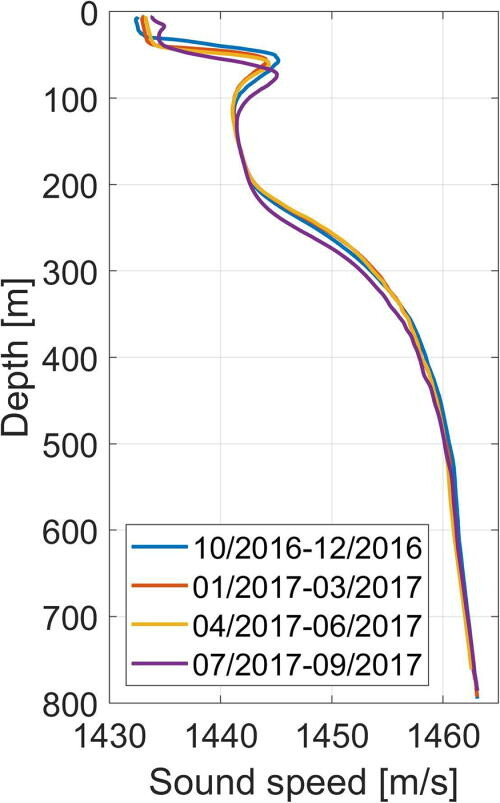
\includegraphics[scale=2]{Figures/ssp.jpeg}
\caption{Sound speed profiles in the Chukchi sea displaying presence of Beaufort duct. Image reproduced with author's permission}
\label{fig_ssp}
\end{figure}

Ambient noise is typically comprised of all the living and nonliving factors generating noise in an environment, essentially the base level of an environment. Underwater, this sound is normally produced at the surface through wind, waves, and precipitation; a portion also comes from geological processes at the sea floor \footcite[]{dziak2015sources}. Marine life communication \footcite[]{ladegaard2021} and anthropogenic operations also contributes to this noise level. In the Arctic, the presence of ice removes air-sea interactions and replaces them with ice driven noise. From icequakes\footcite[]{muller2005singing} and vibrations\footcite[]{kinda2015arctic}, to calving \footcite[]{matsumoto2014antarctic}, cracking\footcite[]{milne1964ambient}, and melting     \footcite[]{glowacki2018intensity} \footcite[]{mahanty2020melt}, ice generates plenty of underwater ambient noise. 

%%%%%%%%%%%%%%%%%%%%%%%%%%%%%%%%%%%%%%%%%%%%%%%%%%%%%%%%%%%%%%
\section{The CANAPE Experiment} \label{intro_canape}

The Canada Basin Acoustic Propagation Experiment (CANAPE) was a yearlong acoustic recording operation conducted from 2016 to 2017 in the Chukchi Sea and Shelf as part of a investigation conducted by the Woods Hole Oceanographic Institution (WHOI) into the Beaufort Duct. There were two facets to this experiment, the deep water Canada Basin (DW-CANAPE) and the shallower water Chukchi Shelf (SW-CANAPE) \footcite[]{ballard2020yearlong}. The acoustic data for this thesis specifically comes from SW-CANAPE.

For SW-CANAPE an array was deployed at the site as seen in \autoref{fig_location}. The specific locations and depths can be seen in \autoref{table_location} It consisted of five several hydrophone recording units (SHRU(s)). Each SHRU had four channels in a vertical line array and also contained temperature and pressure sensors. These channels were deliberatly placed at the depth of the Beaufort Duct to amplify its effects. Data from SHRU1 and SHRU5 are used in this analysis.

\begin{table}
  \centering
  \begin{tabular}{|| c c c c||}
    \toprule
    \textbf{SHRU}  & \textbf{Latitude N}  & \textbf{Longitude W}  & \textbf{Water Depth m}\\
    \midrule
      \texttt{WHOI SHRU 1}  & 72° 54.4123’ & 159° 01.0840’ & 302 \\
      \texttt{WHOI SHRU 2}  & 72° 45.2347’ & 158° 16.3243’ & 308 \\
      \texttt{WHOI SHRU 3}  & 72° 40.6924’ & 157° 54.6493’ & 303 \\
      \texttt{WHOI SHRU 4}  & 72° 36.6582’ & 157° 32.2475’ & 301 \\
      \texttt{WHOI SHRU 5}  & 72° 45.4580’ & 157° 29.2442’ & 445 \\
    \bottomrule
  \end{tabular}
  \caption{%
    Table of SHRU mooring locations and depths
  }
  \label{table_location}
\end{table}

\begin{figure}[ht]
\centering
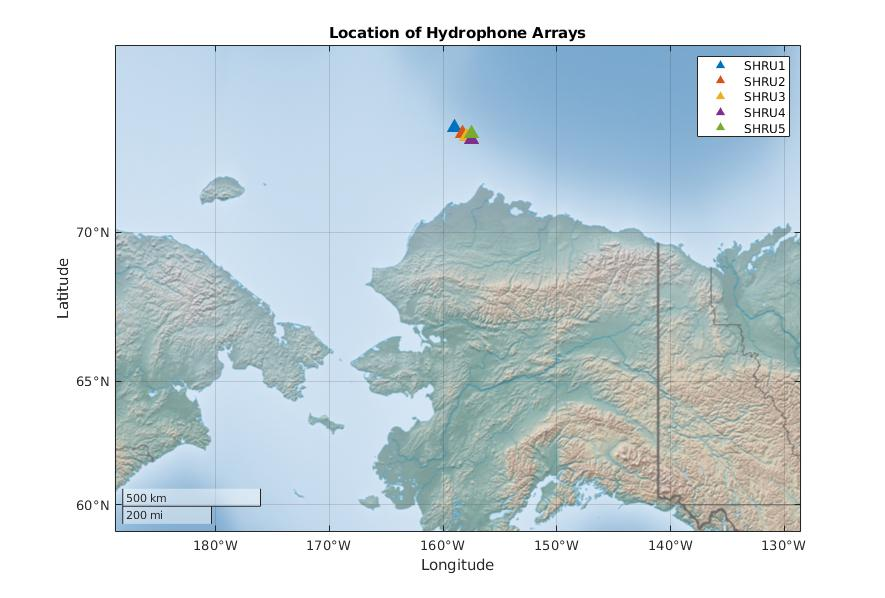
\includegraphics[scale=0.5]{Figures/west_bigmap.jpg}
\caption{Location of SHRU(s) on the Chukchi Shelf}
\label{fig_location}
\end{figure}


As the Canada Basin is an area of particular oceanographic interest, other experiments were ongoing in the region during CANAPE. The University of Delaware's oceanography moorings were also deployed on the shelf, contributed to the overall understanding of the region. Temperature profiles from this experiment helped verify the presence of the Beaufort Duct. \footcite[]{ballard2020temporal} An experiment in DW-CANAPE did create signal interference in the collection of noise by CANAPE, but were rejected in the data processing. \footcite[]{Bonnel2021} 


%%%%%%%%%%%%%%%%%%%%%%%%%%%%%%%%%%%%%%%%%%%%%%%%%%%%%%%%%%%%%%
\section{Data}

\subsection{Acoustic Data Collection} \label{intro_data_col}

\subsubsection{CANAPE Sources}
Acoustic data for this analysis came from SHRU5 and SHRU1 which were 50 km apart; \autoref{sec_probsnstat} contains only SHRU5 data while \autoref{chap_spacial} includes both SHRU(s). Each of the SHRU(s) were placed in the Beaufort Duct with channels 2.5 m apart, ranging from 163 to 170.5 m. The deepest channel at 170.5 m  was used for SHRU5 and the 163 m channel was used at SHRU1. The sampling rate of the SHRU(s) was $f_{s}=3906.2 Hz$ and was recorded continuously through the entire time period. This significant quantity of raw data was then transformed into acoustic products like ambient noise levels. 


\subsubsection{Processing of Acoustic Data}
In order to compute the estimated ambient noise levels, this project assumes the construction of ambient noise to be the coinciding levels of background sound and transient noise. Acoustic data was put in the spectral domain and power spectral densities (dB re 1 $\mu Pa^{2}/Hz$) produced. Then, Ambient Noise Levels (ANL) in dB re 1 $\mu Pa^{2}/Hz$ were created \footcite[]{carey2011ocean} by manually removing data containing transient signals \footcite[]{roth2012underwater}. A short description of the processing done on the CANAPE data is as follows.

The method used to create this ANL analysis derives from a previous study of ambient noise \footcite[]{bazile2013under} by an author of a CANAPE preliminary study\footcite[]{Bonnel2021}. Acoustic data was divided into non-overlapping 7 minute snapshots and then a short time Fourier transform (STFT) was performed with a sliding window of 62.5 ms and 50\% overlap. This short window has a low frequency resolution around 15 Hz but is deemed suitable for the bands of frequency analyzed. It rejects short transient signals less than a few minutes long, which removes the interference of other experimental sources mentioned in \autoref{intro_canape}. ANL is then computed using the 15th percentile of each frequency bin \footcite[]{huillery2008description}, and this process is repeated on every snapshot. Therefore, the resulting ambient noise dataset has an entry for every 7 minutes.

% Following Bartlett's method of the averaged periodogram \footcite[]{bartlett1948smoothing}, a PSD estimate was calculated using the average of the square moduli from the STFT. Long-term spectral average (LTSA) in $\mu Pa^{2}/Hz$

These ambient noise datasets were computed for 50 -1900 Hz across the whole time period. Each frequency band is 50 Hz wide and centered on frequencies from 50 to 1900, 50 Hz apart, for a total of 39 frequency bands. The range was chosen as the original sampling rate ($f_{s}$) of the SHRU(s) is  3906.2 Hz; by the Nyquist sampling frequency, the maximum reliable frequency that can be analysed is 1951.

%%%%%%%%%%%%%%%%%%%%%%%%%%%%%%%%%%%%%%%%%%%%%%%%%%%%%%%%%%%%%%%%%%%
\subsection{Environmental Data} \label{intro_env_info}

Assuming that the ambient noise had mainly environmental drivers, especially under ice, data was acquired for primary environmental factors. In addition the presence of ice coverage helped to delineate the acoustic environments for comparison during analysis. Since part of the focus was on the effects of the Beaufort Duct on the soundscape, determining when it was present greatly mattered.
%%%%%%%%%%%%%%%%%%%%%%%%%%%%%%%%%%%%%%%%%%%%%%%%%%%%%%%%%%%%%%%%%%%
\subsubsection{Ice Coverage} \label{intro_env_ice_cov}

Ice coverage (IC) was considered at the acoustic receiver location, as its influence on the duct would be most felt there. IC data originated from the Integrated Climate Data Center \footcite[]{kaleschke2001ssm} and is derived from the Special Sensor Microwave Imager (SSM/I), a remote sensor. The dataset is created using the ARTIST Sea Ice algorithm \footcite[]{spreen2008sea}. It has a daily temporal resolution and a spatial resolution of 12.5 km x 12.5 km. To reduce the influence of weather variations, ICDC applies a 5 day median filter \footcite[]{kern2010climatology}. IC data is a percentage of the area covered in ice at a grid point in space. These ice coverage percentages were then used to denote environmental time periods.

\subsubsection{Ice Drift} \label{intro_env_ice_dri}

Data for ice drift motion (IDM) came from the Ocean and Sea Ice Satellite Application Facility (OSISAF)\footcite[]{osisaf_data} of the European Organisation for the Exploitation of Meteorological Satellite (EUMETSAT) \footcite[]{osisaf_man} and the National Snow and Ice Data Center (NSIDC) \footcite[]{Tschudi2019polar}. IDM data has a spatial resolution of 25 km x 25 km and daily temporal resolution. Data comes from another microwave sensor and an algorithm that merges information from multiple sensors. The 2D vector of points across the whole Arctic are used in cm/s, though this analysis reduces it down to one dimension of km/day for ANL comparison. 

%%%%%%%%%%%%%%%%%%%%%%%%%%%%%%%%%%%%%%%%%%%%%%%%%%%%%%%%%%%%%%%%%%%
\subsection{Three Acoustic Environments} \label{intro_env_split}

Based on data from the \autoref{intro_env_ice_cov}, acoustic data can be separated intro three time segments critical to this study. Points of IC <15\% were deemed 'no ice' and point >85\% were deemed ice covered. The Beaufort duct was assumed to be present from the beginning to the middle of the ice covered period, up until approximately March 8, 2017. \footcite[]{ballard2020temporal} Intermediate values of ice coverage were omitted, and the time periods they covered cut out (November 8-23, 2016 and June 22- July 12, 2017).

For this analysis, the data is split by time into three acoustic environments:
\begin{enumerate}
    \item{'ice with duct': occurs when there is ice present and the Beaufort duct is present. From November 23, 2016 to March 8, 2017}
    \item{'ice without duct': occurs when there is ice present but the Beaufort duct does not exist. From March 9, 2017 to June 22, 2017.    }
    \item{'no ice': occurs when there is no ice or less than <15\% of ice. This environmental time period covers October 22, 2016-November 8, 2018 to June 30,2017-July 12, 2017. The environmental condition of 'no ice' also means that there is no duct.}
\end{enumerate}

These environmental naming conventions are particularly used in the probability and statistics analysis of \autoref{sec_probsnstat} to compare the ambient noise between environments. Occasionally, the moniker 'ice' is used to refer to both 'ice with duct' and 'ice without duct'. The spacial analysis in \autoref{chap_spacial} focuses only on the environment when ice is present, and so encompasses both the 'ice with duct' and 'ice without duct' environments which go from December 1, 2016 to May 30, 2017. 


%%%%%%%%%%%%%%%%%%%%%%%%%%%%%%%%%%%%%%%%%%%%%%%%%%%%%%%%%%%%%%%%%%%
\section{Statistic and Spacial Analysis}

The the chapters the follow, acoustic data will be examined through two different lenses: statistical parameters in \autoref{sec_probsnstat} and spacial correlation in \autoref{chap_spacial}. As methods the for these analyses differ, separate explanations for each will be presented. Through these chapters, we see that the Beaufort Duct raises ambient noise below 1000 Hz, that ANL is highly related across frequencies, and that IDM and ANL correlate through time.

The effects of climate change may mean that eventually there may only be the two environments 'ice with duct' and 'no ice'. Beyond that, the singular ice-less Arctic environment threatens the stability of the region. Knowing the effects and causes of the changes to the Arctic acoustic soundscape prior to their constant presence could be important for future operations and implications on life there. 

% how does one end an introduction??
%%%%%%%%%%%%%%%%%%%%%%%%%%%%%%%%%%%%%%%%%%%%%%%%%%%%%%%%%%%%%%%
% end of introduction
  
%%%%%%%%%%%%%%%%%%%%%%%%%%%%%%%%%%%%%%%%%%%%%%%%%%%%%%%%%%%%%%%%%%%%%%%%
\chapter{Probability and Statistics Analysis} \label{sec_probsnstat}
%%%%%%%%%%%%%%%%%%%%%%%%%%%%%%%%%%%%%%%%%%%%%%%%%%%%%%%%%%%%%%%%%%%%%%%%

%%%%%%%%%%%%%%%%%%%%%%%%%%%%%%%%%%%%%%%%%%%%%%%%%%%%%%%%%%%%%%%%%%%%%%%%
\section{Introduction to Probability and Statistical Analysis} \label{sec_statintro}
%%%%%%%%%%%%%%%%%%%%%%%%%%%%%%%%%%%%%%%%%%%%%%%%%%%%%%%%%%%%%%%%%%%%%%%% this may not be the best name?

% note to self: stats and probs discussion is very independt of sources/whys, think of this as presenting numbers only

As introduced in \autoref{env_info}, ambient noise in the Arctic can be partitioned into three environmental conditions: 'ice with duct', 'ice without duct', and 'no ice.' Each of these acoustic environments has a unique makeup of ambient noise produced by a variety of drivers and affected by the nature of the environment. By expanding the original frequency band, more information is gained of how ambient sound operates under each environment and the differences between them.  

 A broadband analysis of the ambient sound level (ANL) recorded by the SHRUS was performed using the data from SHRU5. To keep consistency with the original analysis \footcite[]{Bonnel2021}, the data for this analysis came from SHRU5, as it had the least self noise compared to other SHRUS. Each frequency band is 50 Hz wide and centered on frequencies from 50 to 1900, 50 Hz apart, for a total of 39 frequency bands. The range was chosen as the original sampling rate ($f_{s}$) of the SHRUs is  3906.2 Hz; by the Nyquist sampling frequency, the maximum reliable frequency that can be analysed is 1951.  These frequencies were divided into the three acoustic environments of 'ice with duct', 'ice without duct' and 'no ice'. % be sure to CLEARLY define these in section before

Though each frequency has some independent qualities, they appear to be quantitatively linked when analyzed using a myriad of different statistics. These statistic quantities ranged from single metrics to comparing probabilities of the entire acoustic environment. While the original paper examined a frequency band around 300 Hz of 250-350 Hz, it can be assumed that this was not the only frequency propagating through the water. As this analysis would suggest, the frequency range of ambient noise under ice is broad in nature, likely influenced by environmental drivers such as shifting ice \footcite[]{ice_enviro}. This discussion will primarily focus on the numerical quantities and probabilities of ambient sound collected during the duration of CANAPE, independent of time and sources.

% how refs cited kind open on mit website, this works


%%%%%%%%%%%%%%%%%%%%%%%%%%%%%%%%%%%%%%%%%%%%%%%%%%%%%%%%%%%%%%%%%%%%%%%%
\section{Probability and Statistical Analysis Methods and Results}
%%%%%%%%%%%%%%%%%%%%%%%%%%%%%%%%%%%%%%%%%%%%%%%%%%%%%%%%%%%%%%%%%%%%%%%%

%%%%%%%%%%%%%%%%%%%%%%%%%%%%%%%%%%%%%%%%%%%%%%%%%%%%%%%%%%%%%%%%%%%%%%%%
\subsection{Correlation Between Frequencies}
%%%%%%%%%%%%%%%%%%%%%%%%%%%%%%%%%%%%%%%%%%%%%%%%%%%%%%%%%%%%%%%%%%%%%%%%

Exploring the relationships between frequencies in probability shows these environmental conditions share a significant amount of distribution of ambient noise for many frequencies. One can infer that the ambient noise is broadband in nature as many of the previous figures show similar or same results through multiple bands of frequency. In \autoref{fig_freq_corr} the correlation between each of the ambient noise levels of each frequency is shown for each of the three environmental conditions. It is worth noting that the p-value for each of the correlations is an identity matrix, so the likely hood that the null hypothesis is true is zero percent; The exception is when the same frequency is compared against itself as the p-value is 1. The correlation values range from 0.4758 under the 'ice without duct' condition to 1 when frequencies are compared against themselves. 

Other than the very lowest frequencies, correlation between almost all of the frequency bands is quite high, lending credit to the idea that ambient noise encompasses many frequencies.  Each environmental condition does act differently when high and low frequencies are compared to each other, resulting in different shapes of the correlation graphs. The 'no ice' condition has distinct bands of correlation around 0.7 and 0.9 for the 100-200 Hz and 200-300 Hz comparisons; elsewhere is is approximately 1, resulting in a box-shaped block of high correlation values. 'No ice' has the largest area of high correlation values compared to 'ice without duct' and 'ice with duct'.

% not entirely sure if i am able to speculate as to why this is, this is just how it is
The 'ice without duct' condition has minima correlation along the edges of low frequency comparison. From the edges moving inwards, the correlation values increase to nearly 1. There appears to be more correlation between frequencies below 800 when compared to the 'no ice' condition graph, as the 'ice without duct' plot has a less boxy shape and a smoother gradient through correlation values. When high and low frequencies are compared, correlation values range from 0.7 to 0.8. 'Ice without duct' has the least amount of high correlation of \autoref{fig_freq_corr}, and is the least correlated of the three while still showing that many ANL frequencies are very related.

Correlation for the environmental condition 'ice with duct' has the same distinct bands of low correlation at low frequency as the other two graphs, but does not have as distinct of a green band corresponding to 0.7. 'Ice with duct' has a narrower band of high correlation than 'ice with duct' and the middle amount of high correlation values. From about 50 Hz to 1900 Hz correlation values are around 0.9, but once frequencies above 1000 are compared to frequencies below 1000 Hz, correlation drops to around 0.8. While \autoref{fig_freq_corr} definitively shows that many frequencies are closely related, the exact nature of their relationship is not yet shown. Metrics such as mean ANL and pairwise difference display more characteristics of the similarities and differences between the sound through this wide band of frequencies.

\begin{figure}[ht]
\centering
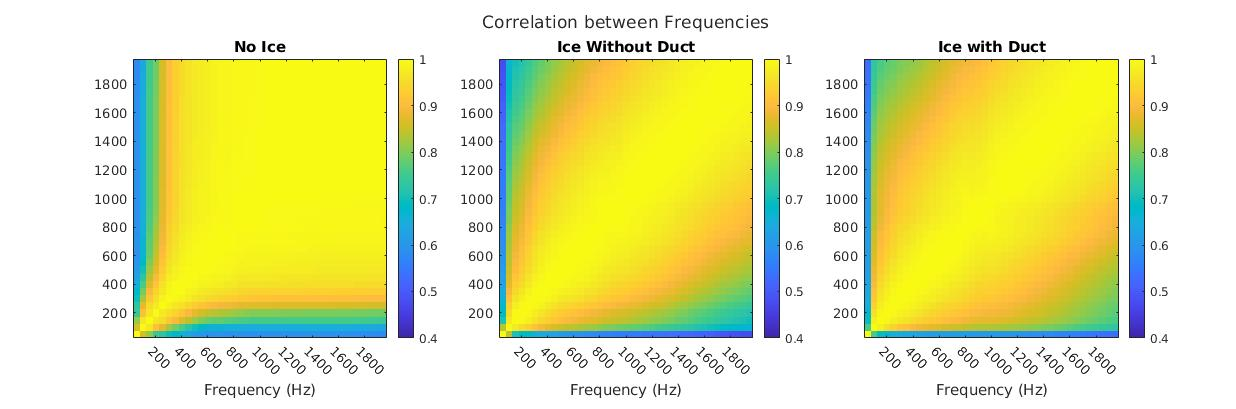
\includegraphics[scale=0.38]{Figures/corr_all_1x3.jpg}
\caption{Correlation between broadband frequencies for }
\label{fig_freq_corr}
\end{figure}

%%%%%%%%%%%%%%%%%%%%%%%%%%%%%%%%%%%%%%%%%%%%%%%%%%%%%%%%%%%%%%%%%%%%%%%%%%%%%%%%%%%%%%%%%%%%%
\subsection{The Ambient Noise Histogram} \label{sec_hist}
One of the simplest ways to visualize the differences between the three environmental conditions is by partitioning the ANL power spectral density (PSD) into histograms. After computing the sound pressure level (SPL) ANL, the bin size for each histogram was vector of 50 values, ranging from the minimum ANL to the maximum ANL of the frequency through all environmental conditions. The average bin size was around 1 Hz, with the highest frequencies having a slightly smaller bin size due to their more limited range. % julien note here?

Histograms were created using the probability density function (PDF) rather than counts to show the normalized likelihood of this ANL occurring. As the acoustic data is finite, an exact PDF is not possible, leading to an estimate function. The equation for this estimate is

\begin{equation} \label{eq:hist_pdf}
 \nu _{i}=\frac{c_{i}}{N \cdot w_{i}} 
\end{equation}

where $i$ refers to the bin, $\nu _{i}$ is the value of the bin, $c_{i}$ is the number of elements in the bin, and \textit{N} is the number of elements in the input data. The sum of all $\nu_{1}$, the bar size, is equivalent or almost equivalent to 1. Therefore, these histograms give the relative probability or makeup of a specific frequency's ANL in dB referenced to  $1 \mu Pa/Hz$ under the three acoustic environment conditions. From this, both the range of ambient noise and the most predominant levels are apparent. To demonstrate the conventions of an interpreting an ANL histogram, looking at a few significant figures showing the differences in acoustic environment levels is more pragmatic than examining 39 separate figures.

%%%%%%%%%%%%%%%%%%%%%%%%%%%%%%%%%%%%%%%%%%%%%%%%%%%%%%%%%%%%%%%%%%%%%%%%%
\subsubsection{Singular Frequency Histogram}
Figure \ref{fig_hist500} is an example of one histogram ranging from 450-550 Hz of the ANL for the three environmental conditions: 'ice with duct',  'ice without duct' and 'no ice'.  The blue histogram is 'ice with duct', the red histogram is 'ice without duct', and the yellow histogram is 'no ice.'  This coloring convention by acoustic environment holds for all statistic figures in this section. The number in the bins is less significant than the distribution of the histograms. 

Similar to the original paper's histogram centered at 300 Hz \footcite[]{Bonnel2021}, this example (\autoref{fig_hist500}) has three distinct peaks for each unique acoustic environment, displaying a key effect on underwater acoustics from changes to the Arctic environment.  It would appear that the quietest ambient levels occur under the 'ice without duct' condition with a highest occurring ANL of about 57 dB. The highest levels of ambient noise belongs to  the 'no ice' condition, with the most common level being around 80 dB. The levels for 'ice with duct' are between 'ice without duct' and 'no ice', with the most common level around 67 dB. 

In terms of shape, the 'no ice' condition histogram is the most normal or Gaussian in form and also has the shortest range from approximately 5-95 dB. 'Ice with duct' seems to have a normal shape, with some right skew and 'ice without duct' is skewed heavily to the right. The two ice conditions has similar ranges from about 62-95 dB, with a matching minimum dB value likely relating the mimimum dB detectable by the SHRUs at this frequency. This minimum detection threshold does change with frequency, as part of the initial setup of the DAQ. \footcite{daq process} %(note that this floor changes with Hz) 

It is commonly said that it is quieter under ice \footcite[]{ice_environ2}, and this figure directly reflects that through the distribution of sound levels in these three different bins. However, this histogram shows that the presence of the Beaufort duct \footcite[]{beaufortduct} increases the presence of louder ambient noise at this particular bandwidth of 500 Hz. When the duct is present, the ANL is likely to be 10 dB higher than an acoustic environment without the duct. Though the range of the two 'ice' conditions is similar,  their distributions are markedly different.  , but this strong difference is only present for a select range of frequencies. 


\begin{figure}[h]
\centering
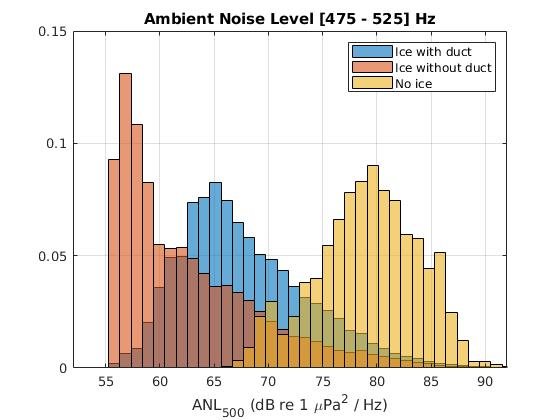
\includegraphics[scale=0.6]{Figures/ANL_500.jpg}
\caption{Histogram of normalized ANL at 500 Hz band for conditions Ice with duct (blue) }
\label{fig_hist500}
\end{figure}


%%%%%%%%%%%%%%%%%%%%%%%%%%%%%%%%%%%%%%%%%%%%%%%%%%%%%%%%%%%%%%%%%%%%%%%%%% order above?
\subsubsection{Multiple Frequencies of Ambient Noise Histograms Compared}
Interpreting one histogram allows its general attributes to be discussed, but more are needed to examine the intricacies of ANL over more frequencies.  For this section, four histograms at frequencies 250, 500, 1000, and 1500 Hz are presented on the same axes in \autoref{fig_selhist} for direct comparison, from 55 to 100 dB on the x-axis, and 0 to 0.25 on the y-axis. Both the distribution and shape of these ANL histograms changes as frequency increases. 

%\textbf{Distribution}

One of the most interesting aspects of the tri-colored \autoref{fig_hist500} is the sharp difference in layout between 'ice with duct' and 'ice without duct'. This phenomena of three separate peaks is only visible from approximately 100 to 700 Hz. The largest stratification between the three bins are between the frequencies of 150 Hz to 500 Hz. Beyond 700 Hz, the red and blue bars tend to overlap as the sound separation dissipates. This three peak ANL could be due to only a band of certain frequencies travelling well or noise in this band being generated into the Beaufort duct \footcite{beaufortduct} , though none of these reasons are certain.

The range of decibel levels covered by the three environmental conditions decreases as frequency increases. In the upper left of \autoref{fig_selhist}, the 250 Hz histogram for all three conditions has a range of almost 50 db, from approximately 57 to 100 dB. In contrast, the bottom right histograms at 1500 Hz cover a diminished range of 55 to 85 dB. The 35 dB long high frequency range is about 15 dB less than the low frequency range. The intermediate graphs of 500 and 100 Hz reflect this decreasing range of decibel values as the bar distribution becomes tighter.

In addition to the diminishing range, there is a general shift down in values for the three environmental conditions. The 'no ice' bars have peak makeup values at 85, 80, 77, and 75 for each increasing frequency. The maximum values of the bars also decrease with frequency for 'no ice', from above 0.1 to 0.75. 'No ice' is the loudest of the three conditions for all frequencies; its peak values are usually 10 to 20 dB more than the others. The other 'ice' environmental conditions do not behave similarly to the 'no ice' trends in ANL distribution.

The red bars for the 'ice without duct' histogram of \autoref{fig_selhist} shift down in peak value while increasing percentage as frequency goes up. At 250 Hz, the maximum bar value is just above 0.05 at 65 dB. When frequency increases for 'ice without duct' the minimum ANL value and maximum bar height tend to align, seen in the 500 Hz and 1000 Hz graphs. In the bottom right corner, the maximum bar height is almost 0.25 at 55 dB for 1500 Hz. 'Ice without duct' is always the minimum amount of ANL out of all three conditions through all frequencies.

The values for the blue bars of the 'ice with duct' histogram are usually somewhere between the values of 'no ice' and 'ice without duct'. 'Ice with duct' is similar to 'ice without duct' at the high frequencies, but differs in the mid to low bands. At 250 and 500 Hz the peak values for 'ice with duct' are between those of 'no ice' and 'ice without duct'. 250 Hz has a 10 dB difference (65-75-85) between each condition, but 500 Hz has a smaller gap between 'ice' conditions (57 to 65 dB) and 'no ice' (65 to 80 db). The red and blue bars align at 1000 and 1500 Hz as the minimum ANL becomes the most predominant noise level. The most predominant value, though not the minimum ANL is around 57 dB. As frequency increases, the maximum bar height also increase, from 0.1 to 0.15, which is less than the 'ice without duct' bar height increase.

\begin{figure}[h]
\centering
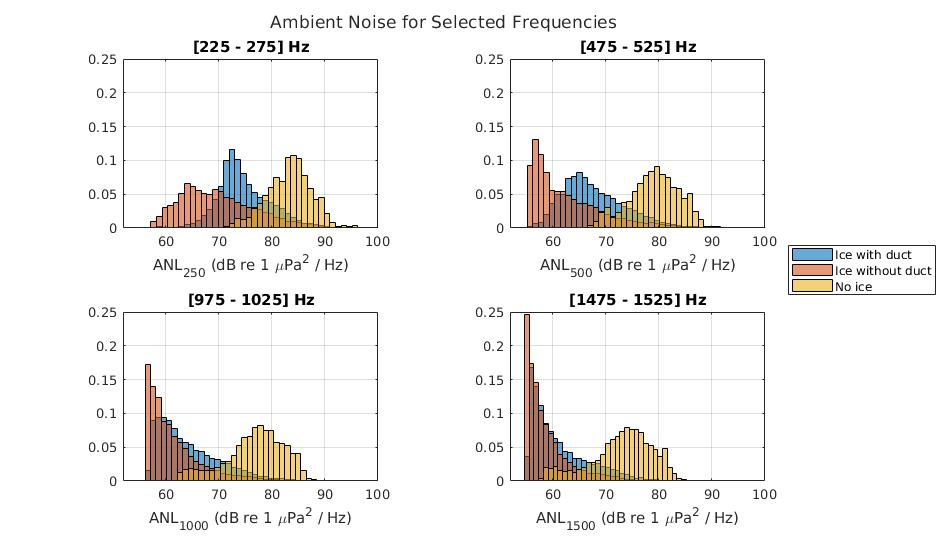
\includegraphics[scale=0.45]{Figures/selected_hists.jpg}
\caption{Histograms of ANL for 250, 500, 1000, and 1500 Hz}
\label{fig_selhist}
\end{figure}
%\textbf{Shape}

The shape of the histograms varies highly throughout the frequencies examined. For 250 Hz and below all three environmental conditions have a fairly normal shape, but above 250 Hz the shapes diverge for all three. The 'no ice' histogram maintains a mostly normal shape through the whole range of frequencies. Without ice to dampen it, ambient sound is likely wind and ocean driven. Toward the highest frequencies, there is a bit of left skew to the 'no ice' histograms, which may be related to the lowered presence of the high frequencies altogether. It does not follow the pattern of the ice environmental condition histograms.

Most of the changes in shape are seen in the red and blue histograms of the ice environment. Above 250 Hz, the 'ice without duct' histogram becomes predominantly right skewed. This right skew for 'ice without duct' emphasizes that the highest occurring noise levels are the lowest values, and that the minimum sound levels occur under 'ice without duct'.  'Ice with duct' is normal in shape from 50 to about 350 Hz, above 500 Hz is begins to be skewed right. At around 900 Hz, the histograms for 'ice with duct' and 'ice without duct' are both right skewed and have heavy overlap. The right skew and overall shift down in values reflect the quieter nature of sound under ice and at higher frequency. It is apparent that there is more sound with ice than without.

% what does it mean



%%%%%%%%%%%%%%%%%%%%%%%%%%%%%%%%%%%%%%%%%%%%%%%%%%%%%%%%%%%%%%%%%%%%%%%%%
\subsection{Average ANL} \label{sec_avg_anl}
Several single numeral metrics for describing the overall behavior of ANL in frequency present trends that cannot be seen through examining histogram graphs alone. \autoref{fig_avg_anl} shows the average ambient noise level of each environmental condition for frequencies 50 to 1900. This average value is taken across the whole yearlong time frame of acoustic data being recorded.  ANL is in dB referenced to $ 1 \mu Pa^{2}/Hz$ are the units of the y-axis and frequency is on the x-axis. The averages for 'ice with duct' are in blue, the averages for 'ice without duct' are in red, and the 'no ice' is in yellow.

A caveat for using the average value as a descriptor is the tendencies to of the data to be skewed, as seen in \autoref{fig_selhist}. A general negative trend in average ANL is present across all three acoustic environment types. 'No ice' behaves linearly while the 'ice' conditions behave more exponentially. Both 'ice' conditions begin to slow the descent of ANL around 600 Hz. There are small increases every four points or so in the data, perhaps caused by the n-50 band being slightly more active at that point. The three lines of \autoref{fig_avg_anl} definitively show that 'no ice' is the loudest of the three conditions for the majority of the frequencies, followed by 'ice with duct'. The lowest levels of ANL typically reside in 'ice without duct'.

When there is no ice, ambient noise can come from a variety of sources including rain, waves, and wind. In addition, shipping in the general area can create a significant quantity of propeller noise as decreased ice leads to higher volume of ship traffic. \footcite[]{ship_traffic} When there is ice, most of the ambient noise in the Arctic when there is ice is generated by the movement of the ice itself - grinding, slipping, and shearing. It would seem the presence of the Beaufort duct increases the average ANL for many frequencies above the normal condition of 'ice without duct'. 
%Things to consider: what else functions in these bandwidths of activity, like whales and other biologic factors? Is what we do going to negatively impact them?



\begin{figure}[p]
\centering
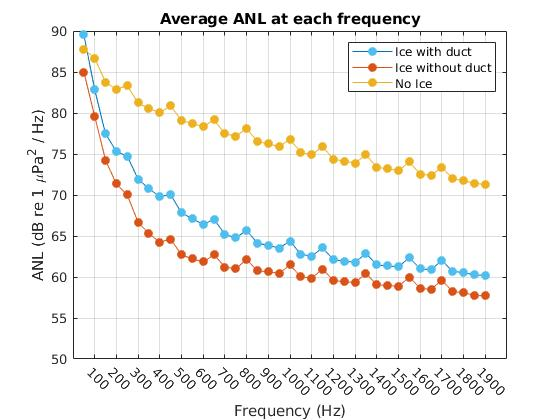
\includegraphics[scale=0.6]{Figures/Average_ANL.jpg}
\caption{Average ANL at frequencies from 50 to 1900 Hz.}
\label{fig_avg_anl}
\end{figure}

% mode cutoof is at 1950, change and LoCK axis corrds to match
\begin{figure}[p]
\centering
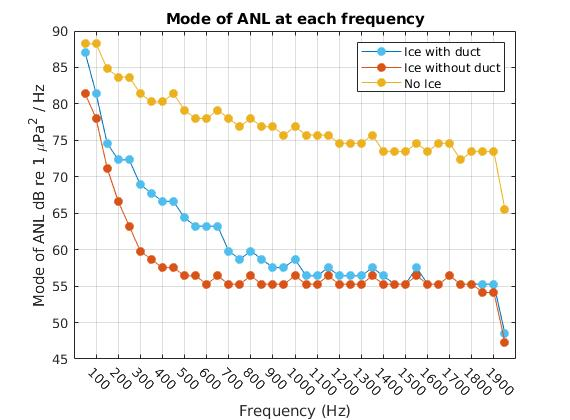
\includegraphics[scale=0.6]{Figures/mode_ANL_allfreqs.jpg}
\caption{Mode or highest occuring bin value of ANL for frequencies from 50 to 1900 Hz.}
\label{fig_mode}
\end{figure}

%%%%%%%%%%%%%%%%%%%%%%%%%%%%%%%%%%%%%%%%%%%%%%%%%%%%%%%%%%%%%%%%%%%%%55
\subsection{ANL Approximate Modes}

Another single metric for describing the general nature of ANL under an environmental condition at each frequency is the approximate mode of the data. While an exact mode was not possible for noise levels with multiple decimal places, an estimate was made using the highest bars of the bin edges in \autoref{sec_hist}. As opposed to the average, this statistic metric leans heavily into the skew of the histogram. Looking at the mode may be better for describing the general trends of each acoustic environment's frequency. When compared, \autoref{fig_avg_anl} and \autoref{fig_mode} display different changes in ANL and frequency. 

% what is going on in mode
The yellow points denoting the modes for 'no ice' have the loudest modes, beginning at almost 90 dB and tapering down to approximately 75 dB. The curve of the 'no ice' line is nowhere near as steep as the ANL modes for 'ice with duct' and 'ice without duct'. The blue points representing the modes of 'ice with duct' begin around 87 dB, close to 'no ice'. A steep drop in decibel mode occurs from 100 Hz to 700 Hz, where the modes begin to plateau around 57 dB.  The red points for the modes of 'ice without duct' behave similarly to 'ice with duct', but the decrease in ANL is more significant at a lower frequency. 'Ice without duct' begins its mode plateau of 55 dB at 500 Hz.

For the lowest frequencies within \autoref{fig_mode}, the different between ANL is less than 10 dB, though by 200 Hz this difference has increased to almost 20 dB. From 50 to 1000 Hz, the modes for 'ice with duct' remain between those of 'no ice' and 'ice without duct'. After this, overlap between the ice conditions occurs. Similar to previous sections, 'no ice' is typically the loudest environmental condition, followed by 'ice with duct', then 'ice without duct'. \autoref{fig_mode} does offer some key differences to this generalized pattern of sound level.

Unlike \autoref{fig_mode}, it appears that 'ice with duct' and 'ice without duct' share their most predominant ANL of 55 Hz. The stratification in their averages is lost when modes are compared, suggesting that at frequencies above 500 Hz, the Beaufort duct is not as prevalent a factor. The mode line for 'no ice' is less steep than the average line for 'no ice', though the two run in generally the same ranges. 

Modes are statistically the highest occurring sound level recorded by the SHRUs, and are therefore the most likely to occur under the environmental conditions presented in the future. In general, all the mode values for each frequency in \autoref{fig_mode} are lower than those of the average values in \autoref{fig_avg_anl}. Comparing these modes numerically could show potential overall ambient noise level changes to the Arctic underwater noise environment.  


%%%%%%%%%%%%%%%%%%%%%%%%%%%%%%%%%%%%%%%%%%%%%%%%%%%%%%%%%%%%%%%%%%%%%%%%%%%%%%%%
\subsection{Pairwise Difference} \label{sec_pairdiff}

Using modes to generalize the ANL for each frequency above 1000 Hz, the ANL for 'ice with duct' and 'ice without duct' are almost the same. Comparing the differences between these modes is a reasonable method for finding a significant metric of the change between conditions. The metric used to make such a comparison is the pairwise difference between these probability distributions. Pairwise difference is the length between two bins at the same frequency between the two environmental noise types being analyzed. 

This metric is not measure of probability but is the difference between the highest probable ANL of each acoustic condition. Pairwise difference in the context of this analysis means the difference between each environmental condition's noise level of the highest histogram bar of the probability distribution, not the highest level of noise recorded. Because the data being compared is a decibel value, the resulting parameter is in terms of noise, and is not a probability. The pairwise difference for this analysis was calculated using the following equation:

%pair_dist_duct_noduct(i)=edges_duct(ind_duct(i))-edges_no_duct(ind_no_duct(i))
\begin{equation}
PD(\mathcal{A},\mathcal{B},\omega)=\mid argmax(\mathcal{H}_{i} [ANL ^{A}(\omega))]-argmax(\mathcal{H}_{i} [ANL^{B}\omega)]\ \mid 	% this is not actual stat distance 
\end{equation}
% argmax of hist-argmaxofhist, repeat equation

Where $\mathcal{H}_{i}$ refers to the histogram bin, $ANL^{\mathcal{A/B}}$ is the ambient noise at an environmental condition, $\omega$ is the frequency of interest, and $\mathcal{A/B}$ refer to the two acoustic environments being compared. As discussed above, $PD$ is not a value of probability, but a decibel measure of the difference between environments. It directly compares two decibel values between two environmental conditons. The x-axis of this graph is frequency in Hz, while the y-axis is the difference in ANL in dB. The three environmental conditions produce three environmental coupling differences, marked by three new point and line colors. \autoref{fig_pairwisedist} labels the environments being compared through pairwise distance with a color combination of environments that are the secondary mixes of the primary colors of \autoref{fig_avg_anl}. Purple is the difference between 'ice with duct' and 'ice without duct', green is the difference between 'ice with duct' and 'no ice', and orange is the difference between 'ice without duct' and 'no ice'


The conditions with the highest overall difference are 'no ice' and 'ice without duct' which are represented by the orange points. This orange line could represent the typical difference between the ambient noise with and without ice prior to the introduction of the Beaufort duct. It begins with a steep increase in dB from 50 Hz to 500 Hz, reaching a top difference of 24 dB at 450 Hz. After, the difference between 'ice without duct' and 'no ice' begins to decrease slightly, hovering around a 20 dB difference from 500 to 1900 Hz.

The middle difference condition comparison is between 'ice with duct' and 'no ice', represented by a green line and points. Beginning with a pairwise difference of 1 dB at 50 Hz, this line also climbs, though not as quickly as the orange line. The difference between 'ice with duct' and 'no ice' reaches a maximum of 19 dB at 900 Hz and settles around 18 dB until 1900. Above 1000 Hz, the pairwise difference for the orange and green lines are very similar, suggesting that there isn't a strong difference between the 'ice with duct' and 'ice without duct' noise levels when compared with 'no ice'. This  similarity between 'ice' conditions is emphasised by the third pairwise difference line.

The third pairwise difference is the conditions with the lowest overall difference of 'ice with duct' and 'ice without duct', represented by purple points. Starting with a 6 dB difference at 50 Hz, there is a small decrease before the pairwise difference between 'ice with duct' and 'ice without duct' maxes out at 9 dB. Following this maxima, the decibel values steadily decline before going near zero from 1100 Hz on. For half of its points, the purple line is more than 15 dB below the other two line's differences.  

This graph shows that the conditions 'ice with duct' and 'ice no duct' are very similar, while the conditions 'ice no duct' and 'no ice' are most different in ANL. One of the most interesting aspects of \autoref{fig_pairwisedist} is the insight into the significant band of frequencies the Beaufort duct seems to affect the most. From 200 Hz to 600 Hz, the highest pairwise difference between these conditions occurs at an average of 8 dB. This significant band is again reflected in the most separation between the orange and green lines occurring from 200 Hz to 600 Hz. The ambient noise of an environment with the duct is higher in ANL than an environment without the duct, resulting in smaller differences when compared to an ice-free environment. However, the stratification between 'ice with duct' and 'ice without duct' does not encompass all frequencies, demonstrated by the overlap between the orange and green lines as frequency increases.

%%%%%%%%%%%%%%%%%%%%%%%%%%%%%%%%%%%%%%%%%%%%%%%%%%%%%%%%%%%%%%%%%%%%%%%%%%%%%%
% figures of total vart dist and pairwise dist
\begin{figure}[p]
\centering
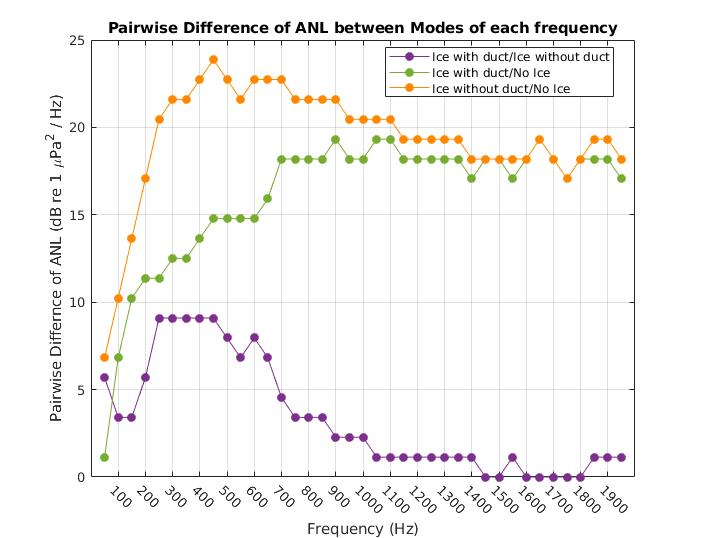
\includegraphics[scale=0.6]{Figures/recolor_pairwise_dist_ANLs.jpg}
\caption{Pairwise distance for frequencies from 50 to 1900 Hz.}
\label{fig_pairwisedist}
\end{figure}

%% FIX LEGEND AGAIN
\begin{figure}[p]
\centering
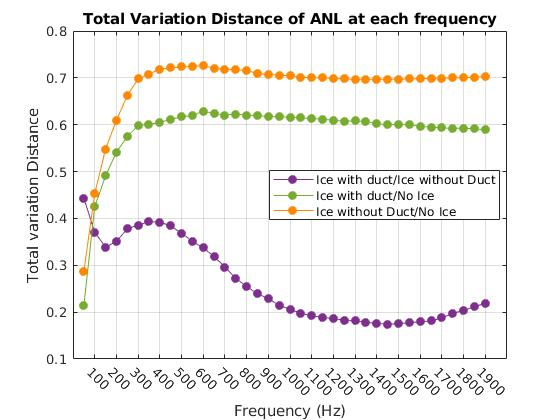
\includegraphics[scale=0.62]{Figures/recolor_total_var_dist_norm_pdf.jpg}
\caption{Total Variation distance for frequencies from 50 to 1900 Hz.}
\label{fig_totvardist}
\end{figure}

%%%%%%%%%%%%%%%%%%%%%%%%%%%%%%%%%%%%%%%%%%%%%%%%%%%%%%%%%%%%%%%%%%%%%%%%%%%%%%%%%%%
\subsection{Total Variation Distance} \label{sec_tvd}
Rather than examine the statistic quantities of each acoustic environmental condition alone, one can compare the relationship between environments by frequency through total variation distance (TVD). This metric shows the likelihood between two probability distributions of acoustic environments. Unlike \autoref{sec_pairdiff}, this metric is a normalized value of probability, not a measure of sound level in decibels. Total variation distance essentially is the absolute area between two curves, showing how likely acoustic conditions will have overlap in their ANL distributions. 

 Total variation distance looks at all the data across all the frequencies, with the count of each bin as a proportion. It takes every value of the probability of that bin and takes the sum of the absolute difference between the two. TDV is not a measure of ANL in dB but a measure of probability of occurrence between two conditions. This data set was normalized using PDF similar to the histograms in \autoref{sec_hist}. For the purposes of this analysis, the total variation distance uses the following equation: 

% equation used for our analysis
%\begin{equation} \label{eq:actualtotvar}
%\delta(Duct, No Duct)=\frac{1}{2} \Sigma \mid Duct(f) - No Duct(f) \mid 
%\end{equation}

\begin{equation} \label{tdv_eq}
    \delta ^{TVD} _{ANL} ( \mathcal{A}, \mathcal{B}, \omega) = \frac{1}{2} \sum _{i} ^{} \mid \mathcal{H}_{i} [ANL^{\mathcal{A}}(\omega)] -\mathcal{H}_{i} [ANL^{\mathcal{B}}(\omega)] \mid 
\end{equation}

where  $\mathcal{H}_{i}$ is the \textit{i}th bin of the environmental condition histogram $\cal{H}$, $\omega$ is the frequency band, and $\cal{A/B}$ refer to the different environmental condition being compared. $\delta$ is the total variation difference between two ANL histograms of different environmental conditions. One number is returned by this equation that sums up the total variation distance between the two conditions. A value of 1 means that two probability distributions are entirely different with no shared ANL values. An output value of 0 means the probability distribution are exactly the same, with the same occurrence of each ANL value.

\autoref{fig_totvardist} uses the same coloring convention as \autoref{fig_pairwisedist}, where purple is the difference between 'ice with duct' and 'ice without duct', green is the difference between 'ice with duct' and 'no ice', and orange is the difference between 'ice without duct' and 'no ice'. The x-axis are TVD values ranging from 0.1 to 0.8. This single metric defining the relationship between two environmental conditions is plotted against frequency fgrom 50 Hz to 1900 Hz, keeping with the rest of the statistic figures.

 The highest variation distance between the conditions ‘ice with duct' and 'ice without duct’ occurs at 50 Hz at a value of 0.44. The highest variation distance between 'ice with duct' and 'No Ice' occurs at 600 Hz with a distance of 0.63. The highest variation distance for 'no ice' and 'ice without duct' occurs at 600 Hz and at a value of 0.72. At no point do the probability distributions for the three environmental conditions not overlap in ANL, though what dB values relate the two are not known. 

The highest TVD line is the relationship between 'no ice' and 'no duct', represented by the orange points. Beginning at 0.3, the line increases from 50 Hz to 400 Hz and then plateaus at a value of 0.7. This indicates that the probability distributions for 'ice without duct' and 'no ice' do not have much in common and are quite different. Looking at \autoref{fig_selhist} validates this, as the red and yellow bars of the respective histograms vary highly in shape.

The middle green line represents the TVD between the environmental conditions of 'ice with duct' and 'no ice'. Similar to the orange line, The green points rapidly increase from 50 Hz to 600 Hz, before declining and plateauing around 0.6 for the higher frequencies. This indicates that the probability distributions for 'ice with duct' and 'no ice' do have some overlap, but are still more than 50\% different from each other. They are not as different as the conditions 'ice without duct' and 'no ice'. 

The lowest TVD values belong to the conditions 'ice with duct' and 'ice without duct', showing that these two conditions are the most similar. The purple line begins below a value of 0.5, which is also the highest value achieved by the purple line. The TVD decrease to 0.35, before a slight increase from 150 Hz to 300 Hz to a TVD of 0.4. Then the points decline under a TVD of 0.2 until 1200 Hz, where there is another slight increase to above 0.2. From 800 to 1900 Hz, it can be assumed that there is a significant amount of similarity in probability distributions between 'ice with duct' and 'ice without duct'. 

Similar to \autoref{fig_pairwisedist}, total variation distance shows that there is a significant band of frequencies where the difference between ambient noise with and without the Beaufort duct is amplified. From 100 to 800 Hz, the purple line representing the difference between ice with duct and ice without duct is higher than the rest of the points. This is also corroborated by the green and orange line increasing in TVD through a similar band of frequency. When the TVD vales for 'ice with duct' and 'ice without duct' are highest, the TVD values for the green and orange points are lowest. Additionally, total variation distance as a whole is lower when the duct is present when compared to an ice-free environment. This suggests that the sound makeup under these two environments is more similar than a traditionally duct-free area, likely attributed to ambient noise with the duct being closer to an ice free Arctic.

%%%%%%%%%%%%%%%%%%%%%%%%%%%%%%%%%%%%%%%%%%%%%%%%%%%%%%%%%%%%%%%%%%%%%%%%%%%
% ADDITIONAL POSSIBLE SECTIONS?
% MAX, min, difference maxmin
% more histograms


%%%%%%%%%%%%%%%%%%%%%%%%%%%%%%%%%%%%%%%%%%%%%%%%%%%%%%%%%%%%%%%%%%%%%%%%%%%%%%
% can always add more like max min covariance more histograms, etc

% the end of statistic section
\section{Probability and Statistics Conclusions}
% a summary of the results from above 'the what it means' section
Using different probability and statistics, certain generalizations about the soundscape of ambient noise in the Arctic can be made. Expanding the frequency of interest from 300 Hz to a significantly wider bandwidth of 1850 Hz increases the understanding of how ambient noise operates in the Arctic sea. The probability distributions of ambient noise show a 45 dB range of sound received between all three environmental conditions. As frequency increases, ANL is likely to decrease, with a minimum ambient noise around 55 dB. A clear difference between louder sound without ice and quieter sound with ice, regardless of duct, exists as well. This decibel difference changes highly with frequency, something not seen before.

From this section, it is apparent that the Beaufort duct has a strong effect on the level of noise under ice in the Arctic. The probability of the duct's presence raising the ambient noise by almost 10 dB is high when compared to a ductless environment. However, this increase in noise is limited to a certain band of frequencies of about 100 to 700 Hz. It is unlikely that the duct would cause the same ANL increase at higher frequencies. This results in similar noise levels above 100 Hz, regardless of whether the duct is present or not.


  
%%%%%%%%%%%%%%%%%%%%%%%%%%%%%%%%%%%%%%%%%%%%%%%%%%%%%%%%%%%%%%%%%%%%%%%%
\chapter{Spacial Analysis} \label{chap_spacial}
%%%%%%%%%%%%%%%%%%%%%%%%%%%%%%%%%%%%%%%%%%%%%%%%%%%%%%%%%%%%%%%%%%%%%%%%

%%%%%%%%%%%%%%%%%%%%%%%%%%%%%%%%%%%%%%%%%%%%%%%%%%%%%%%%%%%%%%%
\section{Introduction to Spacial Analysis} \label{sec_intro_spac}

% note difference between last section and this section, were gonna focus a lot more on environment os buckle up
In \autoref{sec_probsnstat}, ambient noise was split into three distinct acoustic environments in order to asses the overall attributes of each. With the numerical attributes of each environment differing by frequency, it is likely the causes and drivers of this ambient noise differ as well. Acoustic forces behind sound under ice are not the same as the primary powers behind sound in an ice free Arctic ocean. This section will focus on the relationship between ambient sound under ice and the movement of ice itself.

The focus here is exclusively on the ambient noise when ice is present, and does not divide between 'ice with duct' and 'ice without duct' like in \autoref{sec_probsnstat}. The entire time period encompassed by this section is from 01NOV2016 to 30JUL2017, but the highest correlations occurring from 1DEC2016 to 30MAY2017. Time periods with low quality ice data were omitted. Expanding the frequencies examined in spacial correlation analysis emphasizes that all of these frequencies are highly related in sound level, perhaps due to driving source of ice drift. 

While looking at a broadband range of frequencies makes sense for a statistical analysis, looking at the spatial correlation of 38 different frequencies on a map would be cluttered. For ease of computing and viewing, the spatial correlation analysis is limited to the frequencies of 300 Hz, 500 Hz, 1000 Hz, and 1500 Hz. Each band was 50 Hz wide, echoing the conventions of \autoref{sec_probsnstat}. 300 Hz, as opposed to 250 Hz, was retained for comparison with the original analysis; it is known from \autoref{sec_probsnstat} that 250 Hz and 300 Hz are closely related anyhow. While a band around 50 Hz was examined, the low frequencies behaved more erratically than all the other frequencies. This is reflected in the statistical analysis above as the 50 Hz data points are usually different and it can be assumed low frequencies have different acoustic drivers. 

%%%%%%%%%%%%%%%%%%%%%%%%%%%%%%%%%%%%%%%%%%%%%%%%%%%%%%%%%%%%%%%%%%%%%%%%
% seriously why do all my titles sound terrible
\section{Spacial Analysis Methods and Results}
%%%%%%%%%%%%%%%%%%%%%%%%%%%%%%%%%%%%%%%%%%%%%%%%%%%%%%%%%%%%%%%%%%%%%%%%


%%%%%%%%%%%%%%%%%%%%%%%%%%%%%%%%%%%%%%%%%%%%%%%%%%%%%%%%%%%%%%%%%%%%%%%%%%
\subsection{Spacial Correlation between Ice Drift and ANL Method} \label{sec_corr_method}

As described in \autoref{intro_env_info}, the time periods over which the variables of ambient noise and ice drift magnitude (IDM) are 7 minutes and 24 hours respectively. To make the two comparable, ANL was decimated to match the sampling rate of the IDM. Since, the exact metrics of ANL and ice drift cannot be directly compared due to their different units, normalized values for both variables were computed using z-scores and then correlated over specific time periods. 

Correlation was calculated at each point of the IDM map for a 2 month long period of time centered on $t_{0}$; each 2 month long time period center is separated by two weeks, leading to sliding windows with 75\% overlap in time. \parencite{Bonnel2021} The equation to correlate these two metrics is 

\begin{equation}    \label{eq_spacialcorr}
    M(x,y,t_{0})=\Gamma [n(t_{0}),d(x,y,t_{0})]
\end{equation}
 
where $x$ is latitude, $y$ is longitude, $d(x,y,t_{0})$ represents the IDM time series for the time period centered on $t_0$ at position $(x,y)$, $M$ is the correlation map matrix, $n(t_0)$ is ANL during the 2 month long time period centered on $t_0$, and $\Gamma$ is the Pearson correlation function. Correlation coefficients with a $p>0.05$ were removed from the map. Correlations were calculated for various ANL frequencies using data from both SHRU1 and SHRU5, as discussed in \autoref{sec_spa_corr_freqs} and \autoref{sec_corr_shru}.%ref sections or not bc they all use this method

% describing how its plotted one time

For the figures of \autoref{sec_spa_corr_freqs} and \autoref{sec_corr_shru}  the left column shows a colormap of the correlation coefficients. Land is included on the map for frame of reference. The red X represents the point of maximum correlation while the black X represents the position of the SHRU. Where the value of $p\leq0.05$ or if there is no IDM data, the map is white. 

Typically, the correlation color spread is centered on the red X, but isn't confined to one shape as seen in the bottom maps of \autoref{fig_300_16DEC} and \autoref{fig_1500_16DEC}. Distant dark spots on the lower end of the colorbar spectrum appear on some of the correlation maps like in \autoref{fig_300_500corr} and \autoref{fig_1000_1500corr}. These dark blue spots represent areas of low correlation where data was present and the p-value significant enough to not be rejected.

The right columns show the normalized time series of 2-day average ANL and IDM at the location of maximum correlation. The blue line is the ANL at that given frequency, which is more continuous than the orange line representing ice drift per day. The maximum correlation value found between the ANL and ice drift is displayed at the top of each time series, corresponding with the red X of the map. Dates are displayed above the maps, as well as labels indicating where the correlation data came from, specific to each section.


%%%%%%%%%%%%%%%%%%%%%%%%%%%%%%%%%%%%%%%%%%%%%%%%%%%%%%%%%%%%%%%%%%%%%%%%%%5


%%%%%%%%%%%%%%%%%%%%%%%%%%%%%%%%%%%%%%%%%%%%%%%%%%%%%%%%%%%%%%%%%%%%%%%%%%
\subsection{Spacial Correlation across Frequencies} \label{sec_spa_corr_freqs}

\begin{figure}[p]
\centering
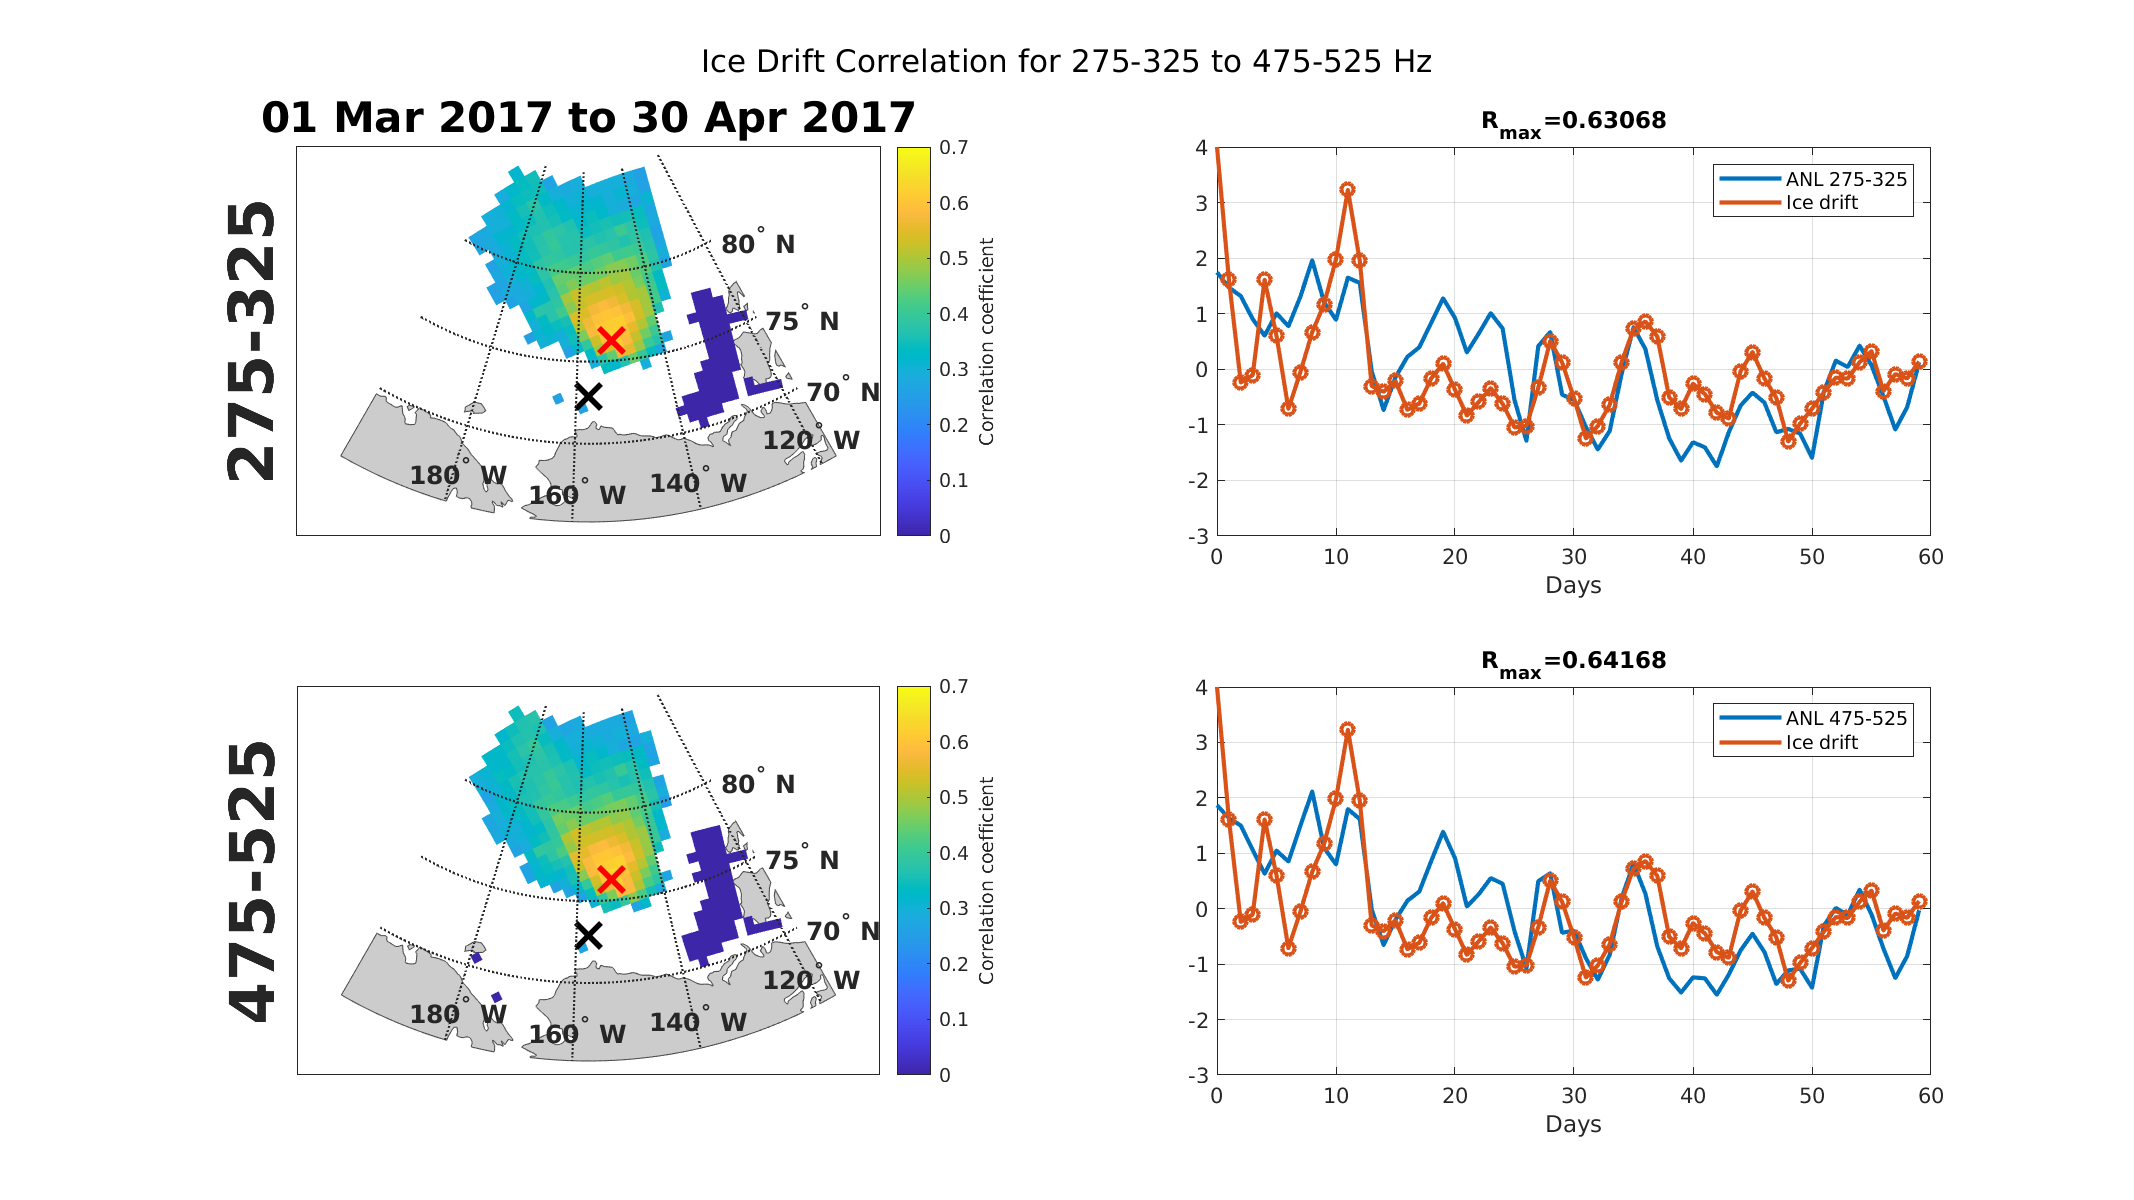
\includegraphics[scale=0.35]{Figures/300_500_spatial_corr_20170301-20170430.png}
\caption{Spacial Correlation map and time series from SHRU5 for 300 Hz and 500 Hz for March 1, 2017 to April 30, 2017}
\label{fig_300_500corr}
\end{figure}


\begin{figure}[p]
\centering
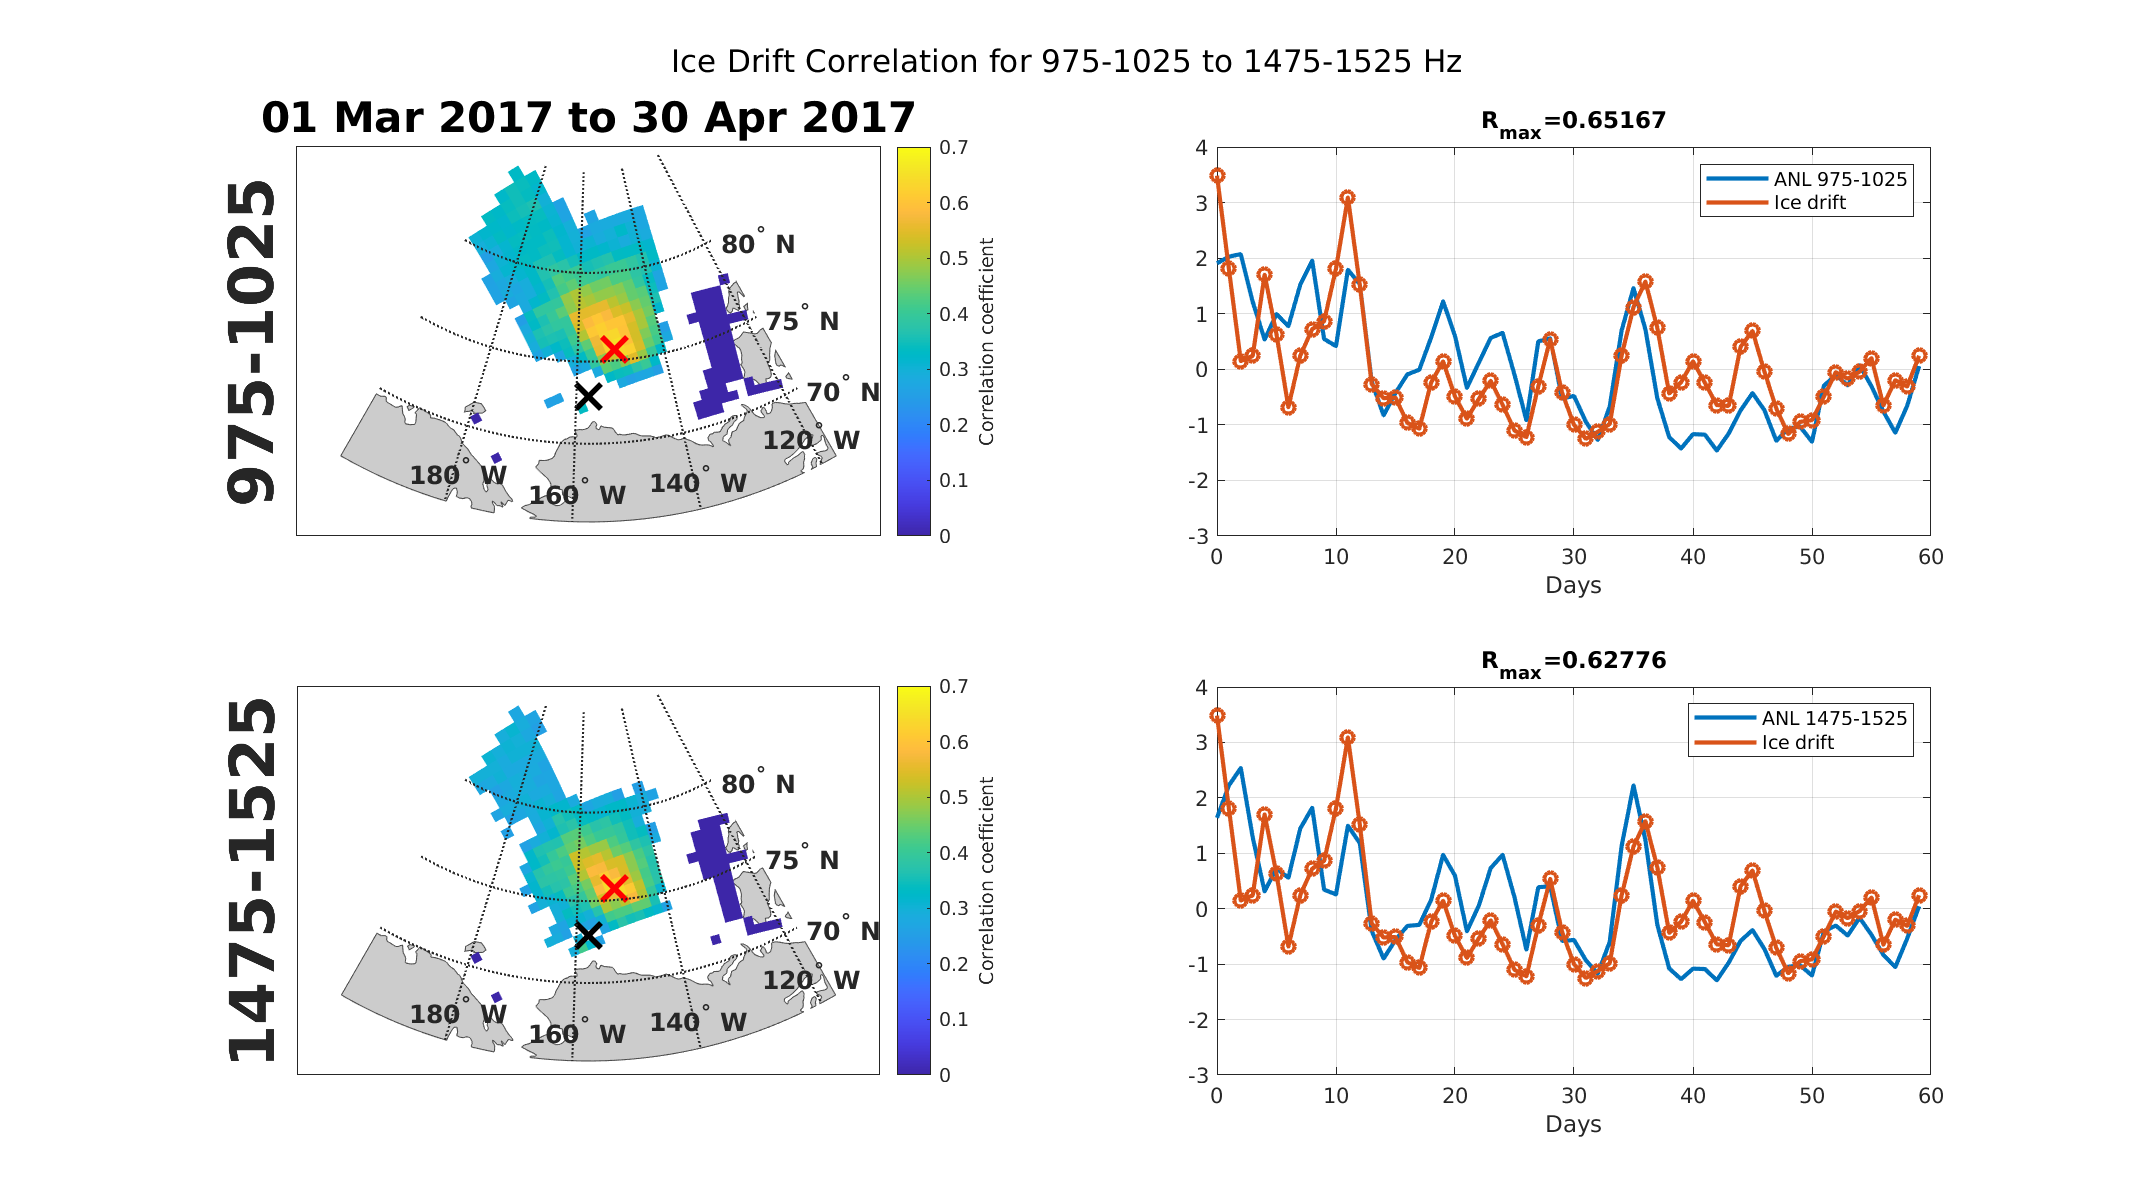
\includegraphics[scale=0.35]{Figures/1000_1500_spatial_corr_20170301-20170430.png}
\caption{Spacial Correlation map and time series from SHRU5 for 1000 Hz and 1500 Hz for March 1, 2017 to April 30, 2017}
\label{fig_1000_1500corr}
\end{figure}

Using the procedures as in \autoref{sec_corr_method}, correlation maps and time-series for different frequencies were plotted together for direct comparison. To keep with \autoref{sec_probsnstat} and because its data usually had more contained colormaps, only data from SHRU5 was analyzed for the major frequencies of 300 Hz, 500 Hz, 1000 Hz, and 1500 Hz. The time period with the highest average correlation coefficient is displayed, but may have not been the actual maximum correlation for every frequency. \autoref{fig_300_500corr} and \autoref{fig_1000_1500corr} contain data from the period of March 1, 2017 to April 30, 2017, which is actually a period when the Beaufort Duct was assumed not present \parencite{ballard2020yearlong}. Even without the helping presence of the Duct, long distance propagation is able to happen and picked up by hydrophones at the depth of the Duct. 

The normalized values of ANL and IDM have similar oscillations in time, with an exception on the fourth day where ANL increases but IDM does not. As theorized before, another environmental acoustic driver like an ice quake could be the cause for this spike in noise. Interestingly, 1000 Hz in \autoref{fig_1000_1500corr} had the highest correlation coefficient, followed by 500 Hz, 300 Hz, then 1500 Hz. From \autoref{sec_peak_prob}, peak probability ANL levels for 300-1500 Hz go from 69-55 dB. Even though sound levels reaching SHRU5 decreased 10 dB over frequency, maximum correlation values were not affected. The drift of the ice generating the sound at a distance creates matching ambient noise in a large breadth of frequencies recorded by the SHRU(s). 

All four spacial correlation colormaps have the same point of maximum correlation for this time period and a surrounding area of high ($\geq 0.4$) correlation. The four also share the same block of minimal correlation from about 140 $\degree$ W to 120 $\degree$ W. Size and shape of the map's correlation spread differ for each frequency. As frequency increases, the number of correlated points decreases, making the colormap smaller. This decrease in correlation size could be due to the lower dB of ANL recorded for 1000 Hz and 1500 Hz, as  sound at higher frequency is likely to attenuate sooner. 

The map spread becomes more abstract in frequency, going from a contained block in \autoref{fig_300_500corr} to having a distended lobe on the northwest corner in \autoref{fig_1000_1500corr}. The area with correlation $>0.3$ in the 300 Hz map translates to the whole colormap of 1500 Hz, but 1500 Hz has lower correlation values. Maximum correlation value does not decrease, but the correlation map seems to be lower and darker in color as frequency increases. So while, strong correlation still exists between IDM and ANL, there are lower coefficients as frequency increases. Lower source levels of ANL and the long distance sound must travel in the surface channel contribute to the decreasing amounts and values of correlation as frequency increases. Less correlation and lower values are likely due to the diminishing presence of 1000-1500 Hz ANL seen in \autoref{sec_probsnstat}.
% hahahah i keept saying blob until i remembered the word lobe exsits

When compared to December plots in \autoref{fig_300_16DEC} and \autoref{fig_1500_16DEC} in the next section, the correlation output and maximum point have both shifted towards the east. This west to east drift of the IDM seems to move the sound source closer then further away from SHRU5, resulting in corresponding correlation coefficients. Looking at the movement of the correlation spread in time across frequencies shows similar patterns, further explored in \autoref{sec_allfreq_map}.

% can probably shave down figure sides to make bigger if needed

%%%%%%%%%%%%%%%%%%%%%%%%%%%%%%%%%%%%%%%%%%%%%%%%%%%%%%%%%%%%%%%%%%%%%%%%%%%%
\subsection{Spacial Correlation across SHRU(s)} \label{sec_corr_shru}

This section uses the same procedures as in \autoref{sec_corr_method} and used above for \autoref{sec_corr_freq}. Ambient noise and IDM correlation exists across hydrophones in the array of \autoref{fig_location}, but correlation values differs due to the different geographic locations of SHRU5 and SHRU1. Two figures are shown demonstrating the correlation between SHRU(s) for different times, created using the methods specified in \autoref{sec_corr_method}. Results from SHRU5 are plotted on the top row, and results from SHRU1 are plotted on the bottom row. 

\autoref{fig_300_16DEC} is a replica of the original 300 Hz examined in the preliminary study \parencite{Bonnel2021} but shown at a different date. \autoref{fig_1500_16DEC} focuses on a frequency band centered around 1500 Hz, as opposed to 300 Hz. In \autoref{sec_corr_freq}, it was definitively shown that ambient noise is highly related through a wide swathe of frequencies. These correlation plots for two distant frequencies reflect this theory for both hydrophones. From this, it can be inferred that ambient noise under ice is similar in frequency and space, as these distant, separate hydrophones show similar correlations.   % wanted both to prove the matching across time

\begin{figure}[p]
\centering
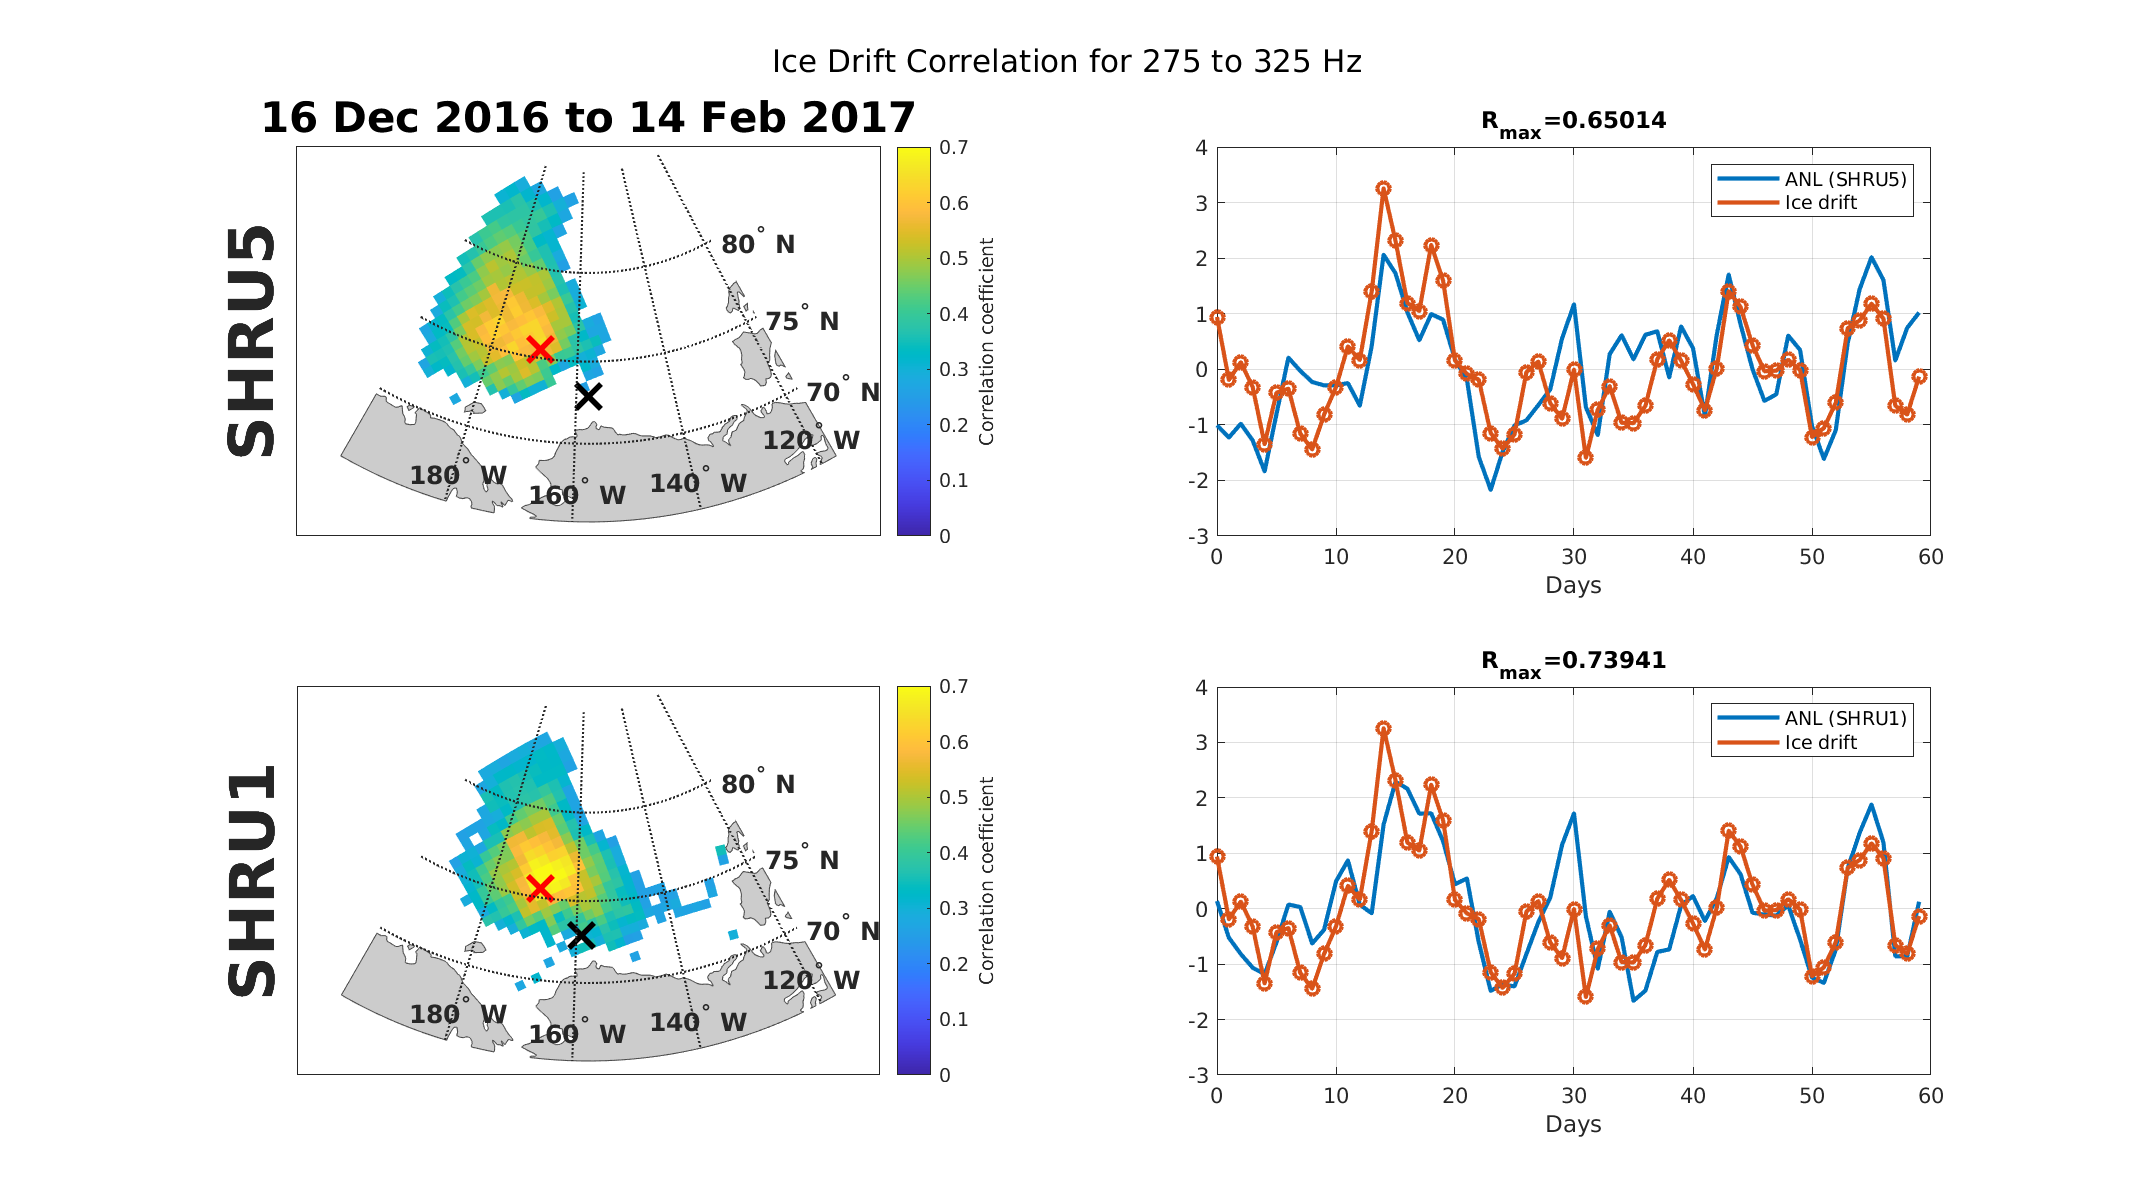
\includegraphics[scale=0.35]{Figures/300_spatial_corr_20161216-20170214_275_325.png}
\caption{Spacial Correlation map and time series for 300 Hz between SHRU1 and SHRU5 for Decmber 16, 2016 to February 14, 2017}
\label{fig_300_16DEC}
\end{figure}

\begin{figure}[p]
\centering
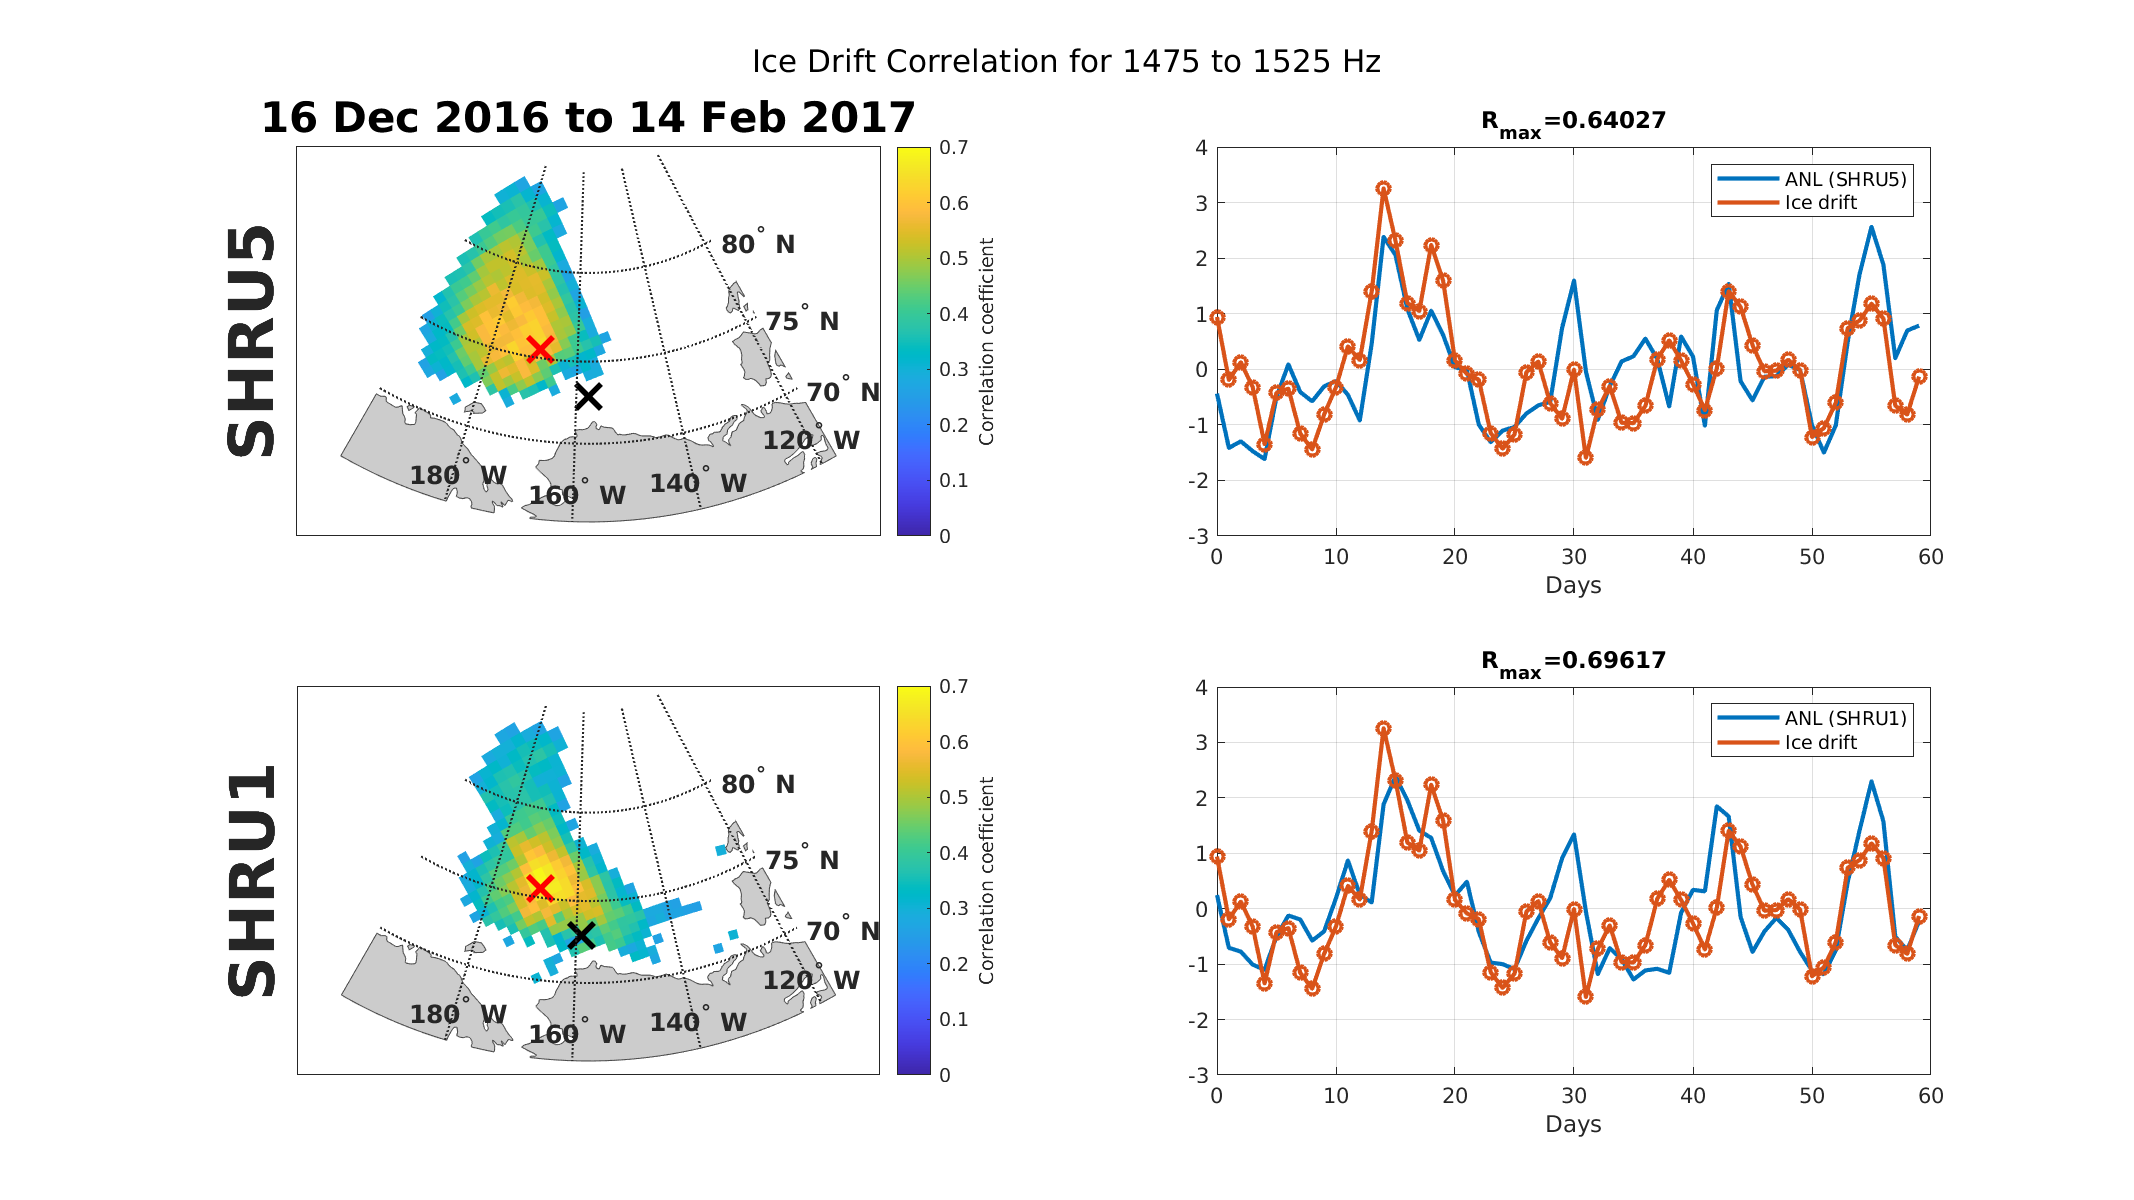
\includegraphics[scale=0.35]{Figures/1500_spatial_corr_20161216-20170214_1475_1525.png}
\caption{Spacial Correlation map and time series for 1500 Hz between SHRU1 and SHRU5 for 16DEC2016-14FEB2017}
\label{fig_1500_16DEC}
\end{figure} 

% timeseries analysis
Looking at the results for two frequencies across two hydrophones leaves no doubt that ANL and IDM are closely linked. At first glance, these two figures seem almost identical, which is beneficial for proving the hypothesis that related ambient noise is caused by shared sources. A cursory observation of \autoref{fig_300_16DEC} and \autoref{fig_1500_16DEC} reveals that normalized ANL and IDM in time is virtually the same for both frequencies. Based on \autoref{fig_timeseries} and \autoref{sec_corr_freq}, normalized ANL for every frequency is almost the same when ANL oscillations aligned. Similarly, normalized IDM looks similar even if the point of maximum correlation is different for every map. Assuming the ice is essentially one interconnected sheet, especially during the winter, movement of the ice would be linked.  


%map analysis
The maps for SHRU5 and SHRU1 for 300 Hz and 1500 Hz are not the same due to the \textasciitilde 50 km between the two recording units, but the area of higher correlation for all four maps is in the same general spot. As SHRU5 seems to be closer to the environmental driver, its correlation maps are tighter for both \autoref{fig_300_16DEC} and \autoref{fig_1500_16DEC}; the correlation maps for SHRU1 are a little more spread out due to extra distance and interference travelling sound would likely experience. Due to these shared attributes, the source of the noise is likely a single cryogenic driver of drift creating most of the received acoustic data during this time period. 

For the most part, oscillations in IDM and ANL at the maximum correlation coordinate match. However, there are times when increases in normalized ANL, such as around day 25, do not have a corresponding increase in IDM. Some alternate source like other types of cryogenic activity \parencite{collins2019acoustic} or biological activity may be affecting some frequencies of the ambient sound at this time. It is interesting to note that ice is more of a distributed source or a plane source than a point source and modelling as a point source isn't entirely realistic to the environment. As Arctic ice changes with time, current, and temperature, the correlation between ANL and IDM changes as well. These changes in time will be examined further in \autoref{sec_allfreq_map}.

% Note correlation tends to decrease from jan to feb, in march we lose data points for ice drift

% well its missing a title

%%%%%%%%%%%%%%%%%%%%%%%%%%%%%%%%%%%%%%%%%%%%%%%%%%%%%%%%%%%%%%%%%%%%%%%%%%
\subsection{Spatial Correlation For Frequencies in Space}  \label{sec_allfreq_map}
%%%%%%%%%%%%%%%%%%%%%%%%%%%%%%%%%%%%%%%%%%%%%%%%%%%%%%%%%%%%%%%%%%%%%%%%%%
 
\begin{figure}[p]
\centering
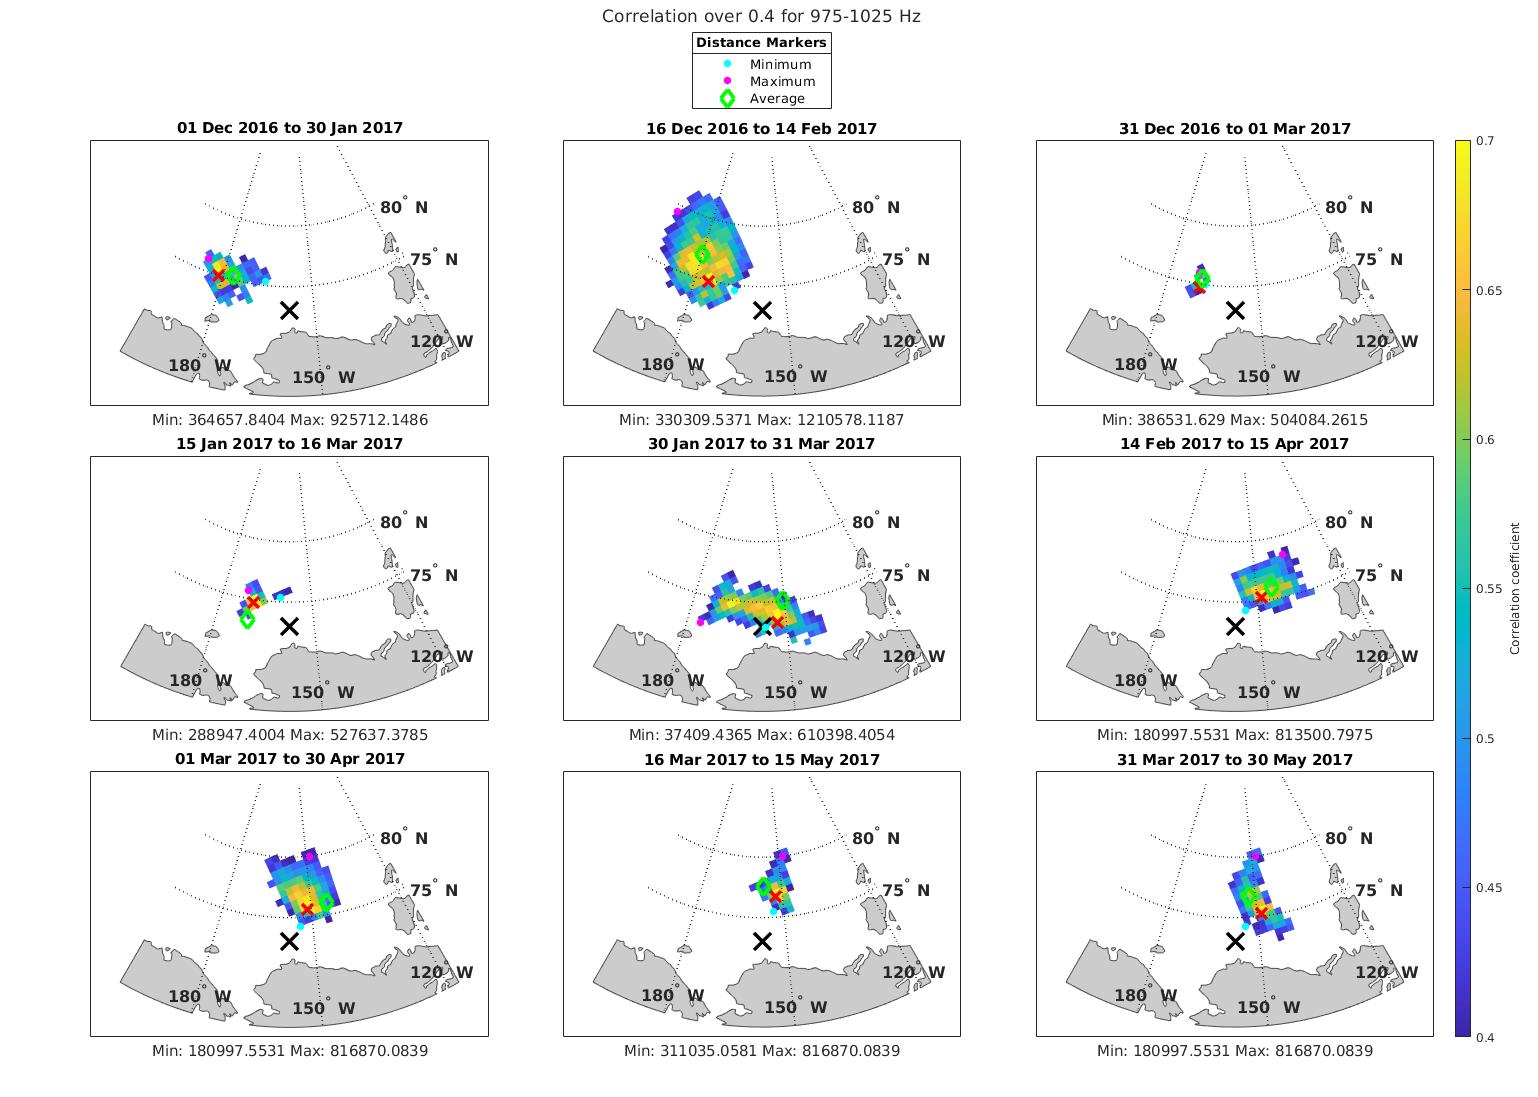
\includegraphics[scale=0.24]{Figures/megamap_noisland_0.4_1000.jpg}
\caption{Maps in time of correlation spread $\geq 0.4$ for band centered on 1000 Hz with markers on minimum distance, maximum distance, and average distance. Note that the colorbar here begins at 0.4, unlike previous maps}
\label{fig_megamap}
\end{figure}

\begin{figure}[p]
\centering
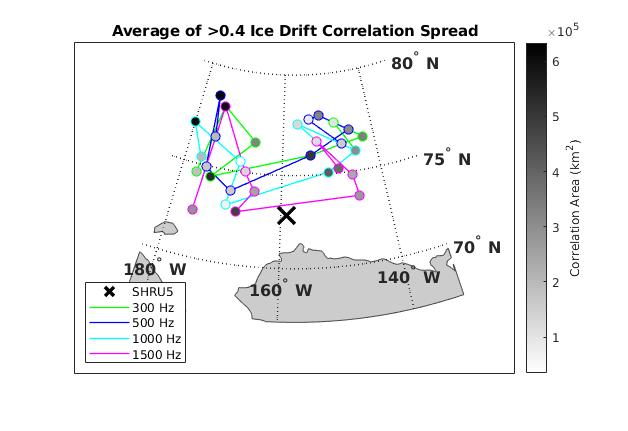
\includegraphics[scale=0.5]{Figures/avg_corr_summary.jpg}
\caption{Average point of $\geq 0.4$ spatial correlation spread and area size for frequencies 300-1500 Hz}
\label{fig_avgmap}
\end{figure}

Now that a relationship between IDM and ANL is known for the frequencies of interest, analysis can be extended to look at the spread of the correlation map over time and examine the strength of the correlation as the ice changes. Taking the correlation maps from \autoref{sec_corr_shru} and \autoref{sec_corr_freq} and cutting off values $\leq 0.4$ for each time period returned new correlation matrices with more significant values. Island outliers distant from the main body of the spread were removed (i.e. single color pixels surrounded by white pixels). For the remaining values $\geq 0.4$, the area of correlation, minimum, maximum, and average distances of the colormap were determined. \autoref{fig_megamap} shows the resulting cutoff correlation map for 1000 Hz through time. Minimum, maximum, and average markers are represented by a blue dot, pink dot, and green diamond respectively. The red X still marks the location of maximum correlation value, and the black X marks the location of SHRU5.

All the cutoff maps for 300 Hz, 500 Hz, 1000 Hz, and 1500 Hz were created and their attributes compared. \autoref{apdx_maps} As anticipated, the size of the $\geq 0.4$ correlation zone in \autoref{fig_megamap} changes with time, affected by the movement of the ice sheet and other environmental factors. For all the frequencies , there is no consistent decrease or increase in size, only variations between the months. Larger correlation areas could be associated with high amounts of IDM over a large area generating sound through the ice sheet itself and into the water. Significant movement events could be a product of storms, currents, or high winds causing shifts in the ice plate. % could also be ice cracks or calving but maybe not in this particular area also not the right time for 

The average distance location points of each frequencies were compiled into one map, shown on \autoref{fig_avgmap}. The colorfill of each average point marker represents the corresponding area of the correlation spread $\geq 0.4$ at that point. The lines of these points are connected to follow drift in time; Green is 300 Hz, blue is 500 Hz, cyan is 1000 Hz, and pink is 1500 Hz. While these points are not labelled with dates, the first point for every frequency begins in the west, and moves generally east. The largest correlation map areas (darkest point fill) tend to cluster in the same places at similar times, which could be large movements in the ice creating a large plane from which ambient noise emanates.

Overall there is a movement of about 1,100 km west to east of the IDM area correlating with ambient noise from SHRU5. This west to east drift in sound is a part of the polar environment affected in part by the influx of current from the Bering strait as well as the circulation of the Beaufort Gyre. Currents coming in from the Bering Sea and the Alaska Coastal Current (ACC) flow closer to the edge of land from west to east, which could affect this ice movement direction. \parencite{Weingartner2005}  The area of correlation could be ice shifted by the ACC or sound could be generated by new ice being pushed against existing sheets. Either way, it is clear that ice drift is part of the source behind ambient noise for many frequencies during this time period. 

%Interestingly, the direction of the Gyre is usually clockwise, meaning the circulation of the ice is usually east to west, opposite of the direction found in the correlation map.



%%%%%%%%%%%%%%%%%%%%%%%%%%%%%%%%%%%%%%%%%%%%%%%%%%%%%%%%%%%%%%%%%%%%%%
\subsection{Distribution of Spacial Correlation through Time}
%%%%%%%%%%%%%%%%%%%%%%%%%%%%%%%%%%%%%%%%%%%%%%%%%%%%%%%%%%%%%%%%%%%%%%

Besides observing the movement of the correlation maps and average points in space, one can also compare the correlation distances in time. Another interesting metric to compare between frequencies are the distance metrics of the spread. \autoref{fig_totalice} shows the minimum, average, and maximum distance of the $\geq 0.4$ correlation spread as a series in time of errorbar-style plots for each frequency. Beginning and ending with the same date as the spacial correlation maps, these plots are a numerical approach to describing the areas where sound is correlated with IDM.Dates on the x-axis are consistent with the end two month long overlapping time period used in \autoref{sec_spa_corr_freqs}

Keeping with the same color convention of the rest of this chapter, the central connected dots represent the average distance from the cutoff correlation spread. The lower and upper bounds of the bar represent the minimum and maximum distances respectively. These distance values range from just a few kilometers to over 1200 km. Similar to \autoref{fig_avgmap} the distance markers vary highly but do not follow any trends in time. 

The four subplots of \autoref{fig_totalice} show matching trends in rise and fall of average distance, but 300 Hz and 500 Hz are more similar than 1000 Hz and 1500 Hz. The length of the bars is highest for 300 Hz and decreases in size through 1500 Hz. Keeping in line with \autoref{sec_probsnstat} the diminishing bar size could be a result of the higher ambient noise levels experienced at low frequencies. The highest distance shared between the four subplots is 1200 km around December 16, 2016. This high spike likely occurred because a large portion of ice was moving and creating sound over a wider area than other time periods.

From \autoref{fig_totalice} the similarities between the correlation of IDM and ANL frequencies over time is apparent as the distance to the source usually aligns. The distance that sound can travel under water with and without the duct is long range for more than just low frequencies. Matching trends in the subplots indicate a shared ambient noise driver in both frequency and time. 

% this title is BAD on the figure
\begin{figure}[p]
\centering
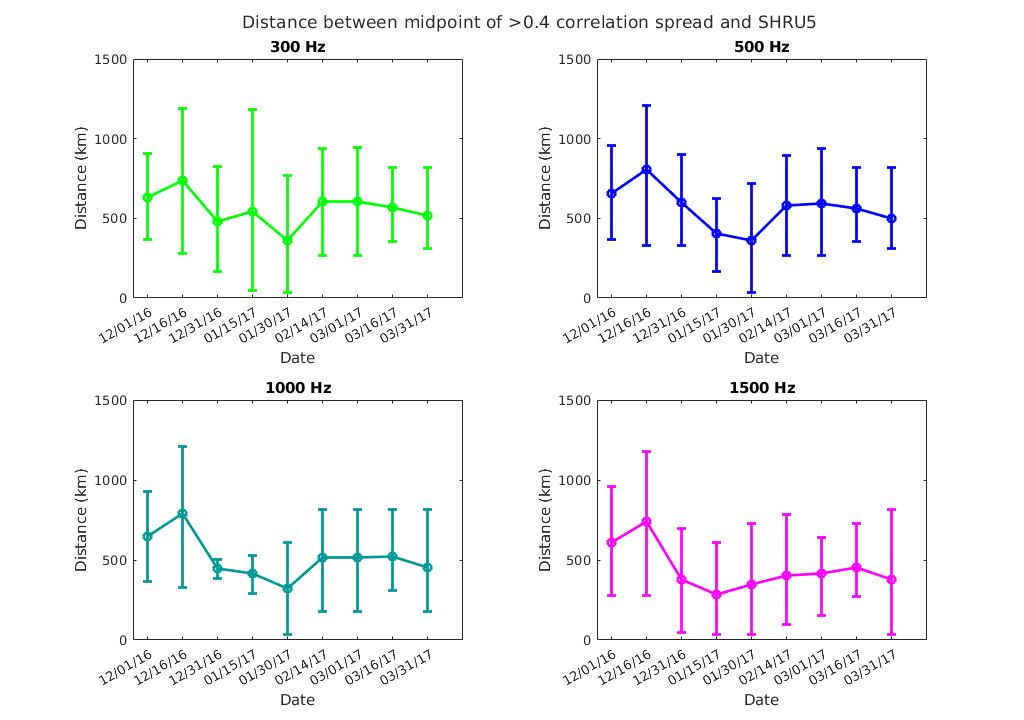
\includegraphics[scale=0.38]{Figures/errorbars_tiled_noisland.jpg}
\caption{Minimum, average, and maximum distance of the correlation spread above 0.4}
\label{fig_totalice}
\end{figure}

% btw the title on this figure is wrong fix dates and make solid lines

\begin{figure}[p]
\centering
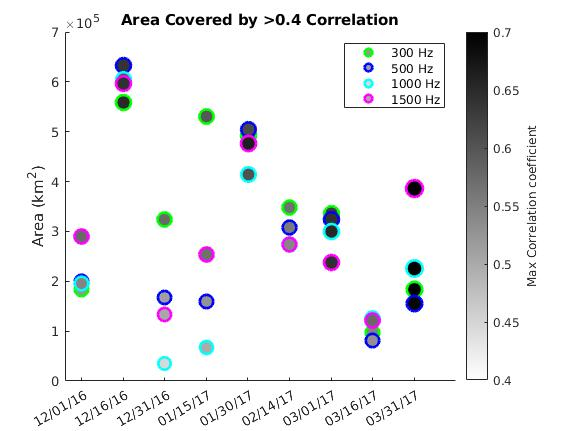
\includegraphics[scale=0.5]{Figures/area_cov_by_>0.4_noisland.jpg}
\caption{Area of correlation spread in km$^{2}$ and corresponding maximum correlation value for frequencies 300-1500 Hz}
\label{fig_maxcorr_dist}
\end{figure}

%%%%%%%%%%%%%%%%%%%%%%%%%%%%%%%%%%%%%%%%%%%%%%%%%%%%%%%%%%%%%%%%%%%%%%%%%%
%\subsection{Spacial Correlation of Frequencies through Time}
% we have combined sections 

Besides looking at the distances from the hydrophone to the correlation map, one can also examine the area of correlation spread as it grows and shrinks through time. \autoref{fig_maxcorr_dist} shows the area of correlation spread in square kilometers, along with the maximum value of correlation at that time as the colorfill of the point. As seen in \autoref{fig_300_500corr} and \autoref{fig_1000_1500corr}, oftentimes these maximum correlation points are in very similar places, leading to overlap in the points. A coloring convention similar to \autoref{fig_totalice} is used.

The area of the correlation spread loosely decreases with time, going from around 600,000 $km^{2}$ to 200,000 $km^{2}$. The formation and shrinking of the ice pack could be responsible for the large to small correlation area differences. Interestingly, there is a pattern of alternation between a stronger and weaker correlation value. For most of the points, a higher value of correlation area coincides with a higher maximum correlation value from the spread.

Most of the points are clustered in a certain area, with an exception from December 2016 to January 2017. Most of the places where the frequencies share similar correlation areas have higher maximum correlation values as well. Continuing with the idea that large movement of large areas of sound creates higher correlation, smaller areas seem to match with lower correlation values. The four frequencies tend to have similar area and correlation values, keeping with the strong relationship between ambient noise frequencies. As these sources are wide and their initial source levels aren't known, this adds complexity to estimating the loss between the received ambient level and ice source. In order to verify many of these results, additional nontrivial modelling is required. 







%%%%%%%%%%%%%%%%%%%%%%%%%%%%%%%%%%%%%%%%%%%%%%%%%%%%%%%%%%%%%%%%%%%%%%%%
\section{Spacial Analysis Conclusions} %summary? conclusion? idk what to call
%%%%%%%%%%%%%%%%%%%%%%%%%%%%%%%%%%%%%%%%%%%%%%%%%%%%%%%%%%%%%%%%%%%%%%%%

%Here, sum up the 'what does this mean of the above'
%
%\subsection{Correlation between Ice Drift and ANL}
During the Arctic winter, the Arctic ice sheet dampens most of the other ambient noise normally heard on open seas. While the acoustic environment is quieter, it is by no means silent as the ice itself becomes the primary source of ambient noise.  Whether the duct is present or not, there is significant long range travel of ambient noise associated with the drift of ice. Ambient noise is captured from these areas and correlated with the drift of ice itself. This steady correlation holds from 300 to 1500 Hz as the ambient sound permeates through all these frequencies.

The size of the correlation map and the distance from SHRU5 to this spread are also linked as a larger area of ice movement creates significant ambient noise able to travel long distances. These areas of ice drift are very large, furthering their ability to send long range sound for many kilometers. Though the size of the area, distance, and the correlation coefficients of the spread between ANL and IDM differ through time, 300-1500 Hz change together. This further demonstrates that underwater ambient noise encompasses many frequencies, and is highly connected to the drift of the Arctic ice sheet. 








  
%%%%%%%%%%%%%%%%%%%%%%%%%%%%%%%%%%%%%%%%%%%%%%%%%%%%%%%%%%%%%%%%%%%%%%%%
\chapter{Conclusions and Future Work}
%%%%%%%%%%%%%%%%%%%%%%%%%%%%%%%%%%%%%%%%%%%%%%%%%%%%%%%%%%%%%%%%%%%%%%%%

%%%%%%%%%%%%%%%%%%%%%%%%%%%%%%%%%%%%%%%%%%%%%%%%%%%%%%%%%%%%%%%%%%%%%%%%
\section{Conclusions from Statistic and Spacial Analysis}
%%%%%%%%%%%%%%%%%%%%%%%%%%%%%%%%%%%%%%%%%%%%%%%%%%%%%%%%%%%%%%%%%%%%%%%%

Exploring the probability and statistical metrics of a broad range of frequencies from 50-1900 Hz improves our understanding of the changing Arctic soundscape. If current warming trends continue, soon the rest of the Arctic may resemble the badly affected Canada Basin in terms of ice loss. Thinking of the Chukchi Shelf as representative of the Beaufort Sea and the Arctic at whole allows for the consideration of the results from this study being found beyond the experimental area.  In focusing on the effects and drivers of ambient noise, we gain some generalizations about the future of the ambient soundscape.

The majority of frequencies in this study were highly correlated with each other in ANL. This suggests that these frequencies have a shared acoustic driver or drivers. Looking at different frequencies in time also showed matching oscillations of ANL, though amplitudes differed by frequency. From looking at the statistics and probabilities of 50-1900 Hz ANL for 'ice with duct', 'ice without duct', and 'no ice', of number of conclusions are gathered. 

Over the course of a year, the ambient levels crossed a 45 dB range of noise shared among the three environments. Maximum noise levels fell as frequency increased, making 55 dB the quietest ANL(s) this area of the Arctic experiences when ice is present. The consistently loudest environment was 'no ice', reaching up to 90 dB at low frequency. Expanding the frequency band showed that 'no ice' shared only 30\% of its  ANL distribution >300 Hz with the 'ice' conditions. We gather that ANL(s) are more similar between lower frequencies.

Significantly, the Beaufort Duct has a pronounced effect on ANL when compared to a ductless environment. A 2-10 dB increase in ANL occurs when the Duct is in the area, but only for frequencies below 1000 Hz. Above 1000 Hz, the probability distributions of 'ice with duct' and 'ice without duct' become indistinguishable. This means the Duct has a greater effect on sounds and signals produced below 1000 Hz, improving their long range conduction underwater. Its continued existence would raise ambient levels across the Arctic as the Beaufort Duct increases its spacial and temporal range.

The sources of this ambient noise are non trivial and complex, creating sound capable of travelling many kilometers underwater. Though it is quieter under ice, there is still plenty of noise created by the ice itself as well as biologic factors. Ice drift movement magnitude and ANL share a strong relationship and correlation through time. This correlation is also shared from 300-1500 Hz, enforcing the idea of frequency correlated noise sharing sources. Correlation can be found across multiple hydrophones at different locations, validating this assumption.

These correlation spreads between IDM and ANL cover thousand of square kilometers with maximum distances beyond 1200 km.  While ANL(s) are known to decrease with frequency, the relationship between IDM and ANL does not fluctuate highly. Correlation $\geq0.4$ exists through all time and frequencies (300-1500 Hz), even as the size and shape of the map spread change. The movement of all correlation maps travels from west to east over time, reflecting the influence of environmental factors like the Alaskan Coastal Current and the Beaufort Gyre. 

IDM is not the only factor behind ambient noise, as other events like melting and calving affect ANL over the duration of the experiment. The conditions of the Arctic are highly favorable for long distance underwater sound through the Arctic facilitated by both the ducts in the water columns and the type of noise radiating from the ice. As these results come from hydrophones within the Beaufort Duct, the levels detected are probably local to the duct's depth range. However, as the Duct exists over much of the Arctic almost all year, increases in noise are not limited to one area in space. The noise levels in the Chukchi Shelf and Canada Basin may be representative of the changing noise levels in the Arctic at large. 
%though about being in duct makes effect bigger



%%%%%%%%%%%%%%%%%%%%%%%%%%%%%%%%%%%%%%%%%%%%%%%%%%%%%%%%%%%%%%%%%%%%%%%%

%%%%%%%%%%%%%%%%%%%%%%%%%%%%%%%%%%%%%%%%%%%%%%%%%%%%%%%%%%%%%%%%%%%%%%%%
\section{Impacts on the Arctic}

\subsection{Biological and Habitat Impact}

The changing acoustic soundscape of the Arctic is already known to have a profound effect on the biology that inhabits the polar seas. The increase in noise that the Beaufort Duct created could affect the critical ecosystem of the Arctic by changing the habits of the life within. Animals that use acoustic communications may change their behavioral patterns to accommodate the duct. Bowhead whales use a frequency band of up to 3000 Hz \parencite{clark1984sounds} and are known to dive around the Beaufort Duct's depth \parencite{simon2009behaviour}. The Beaufort Duct could amplify these whale's acoustic communication ranges, which could for the interaction of more whale pods. However, with higher levels of ambient noise, whale calls would need to be louder. Whether this signal-to-noise ratio compensation is attainable or beneficial to the bowhead population has not yet been studied.

The effects of airgun \parencite{halliday2020potential} and shipping noise \parencite{halliday2017potential} on marine mammals have been studied more than the behavioral response of other vertebrates like fish. Of the many species that reside in the Arctic and bolster the world's fishing economy, few have been studied. Exploring the relationship between shipping and Arctic sculpin was the first study done of this type. \parencite{ivanova2018sculpin} It's now known that shipping drives away Arctic cod \parencite{ivanova2020shipping}, but they are not the only species present. Migratory species like Arctic char that follow ice breakup \parencite{hammer2021char} may have their patterns disrupted by intrusive sound. Though studies have shown that noise pollution negatively affects invertebrates in other oceans \parencite{difranco2020}, little is known about the specific repercussions of noise on Arctic invertebrates.

The continued decrease in ice coverage draws those interested in the natural resources of the Arctic. Increases in noise generated from shipping, drilling, construction \parencite{gering2020aca} and more would exasperate the effects on a region already coping with increased ANL overall. Besides the increased noise, these attempts to exploit the Arctic would result in the destruction of habitats and potential release of substances harmful to the environment, like oil or chemical runoff.


\subsection{Underwater Communication}

There are some utilitarian aspects to the existence of the Beaufort Duct, if it continues to pervade the Arctic ocean over the years. The deeper sound duct opens the door to increased long range underwater communication at lower power than before \parencite{freitag2015underwatercomms} . As ambient noise is driven by cryogenic factors from far away (>500 km); the Beaufort Duct is already known to be conducive to long range proportion. This opens the door to various scientific and anthropogenic-related interests.

The Arctic will need continued monitoring as the effects of climate change continue to reduce the ice pack. This naturally leads to a waterfall of other changes in temperature, chemical makeup, and more which all affect how the Arctic can be studied. Environmental factors will need to be measured regularly in order to keep an active and correct picture of the Arctic, needed for any operations in this area \parencite{Schmidt2016commnav} . Proposals for monitoring arrays, float networks, and autonomous vehicles could benefit from the Duct's sound conducting properties by improving communications and reducing power consumption \parencite{kukulya2016development}. The increased human presence would certainly increase the amount of likely obtrusive man-made sound.



%%%%%%%%%%%%%%%%%%%%%%%%%%%%%%%%%%%%%%%%%%%%%%%%%%%%%%%%%%%%%%%%%%%%%%%%
\section{Potential for Future Work}


For this project, some transmission loss estimates were made using the modal propagation tool KRAKEN to try and replicate the paths noise generated by IDM would travel. This modelling, though not entirely successful, helped create some ideas for future projects. One of the key issues in modelling the source of the noise is that assuming ice generates sound as a line source or a point source is invalid. The ice sheet acts more as a 2D distributed source, generating sound that propagates into the water column and through the ice itself, essentially travelling in two directions. The other issue is that the source level of drift noise isn't quite known; its likely a combination of slipping and grinding as the ice shifts around.

Future iterations of this work could explore estimating the source level of IDM and applying that to a distributed source. Variables such as source level, the presence of the duct, and the size of the source could be altered to try and reproduce or violate the received sources in this study. Another method of validating the correlation between ANL and IDM is beamforming using data from multiple channels. This beamforming would be twofold, as each SHRU(s) is a four channel vertical array and the whole SHRU system a larger horizontal array of 5 SHRU(s). Beamforming would give insight to the directionality of sound captured, to verify is noise was coming from the area of correlation. Additionally, there is a triangular aspect to the SHRU array, as seen in \autoref{fig_location}. Time delayed responses from the triangular and linear portions of the array can be used to estimate the location of the source itself, though this method may be more suited for transient events.

Another potential idea for the future is another version of CANAPE, where some hydrophones are placed in the Duct, and some outside of it. These would provide data about sound levels both in and out of the Duct at the same time, which could be important to communications, modeling, and operations in the area. Especially as the Beaufort Duct has become a prevalent feature of the Arctic soundscape, knowing the challenges and understanding how to operate in the new environment is important for the future of Arctic research.


%%%%%%%%%%%%%%%%%%%%%%%%%%%%%%%%%%%%%%%%%%%%%%%%%%%%%%%%%%%%%%%%%%%%%%%%
\section{Importance of the Arctic}

Greater knowledge about the effects of climate change on the Arctic is critical to try to preserve this key environment of earth. These effects on this Arctic habitat fundamentally affect the life dependent on this region, including many species of fish, whales, and humans. Small changes to the environment here will surely spread through the complexities of the world ocean. The more that is known about the implications of ambient sound in an area previously covered by ice, the more the scientific community and world at large can do to try and mitigate these changes. Climate change is here to stay, and reversing the impacts of it nigh on impossible. Policies about conservation, shipping, and the exploitation of the Arctic are unfortunately one of the few ways this area can be protected from the encroaching interests of the world.

% This ensures that the subsequent sections are being included as root
% items in the bookmark structure of your PDF reader.
\bookmarksetup{startatroot}
\backmatter

  \begingroup
    \let\clearpage\relax
    \glsaddall
    \printglossary[type=\acronymtype]
    \newpage
    \printglossary
  \endgroup


  \printindex
  \printbibliography



\end{document}

%%%%%%%%%%%%%%%%%%%%%%%%%%%
